
% Default to the notebook output style

    


% Inherit from the specified cell style.




    
\documentclass[11pt]{article}

    
    
    \usepackage[T1]{fontenc}
    % Nicer default font (+ math font) than Computer Modern for most use cases
    \usepackage{mathpazo}

    % Basic figure setup, for now with no caption control since it's done
    % automatically by Pandoc (which extracts ![](path) syntax from Markdown).
    \usepackage{graphicx}
    % We will generate all images so they have a width \maxwidth. This means
    % that they will get their normal width if they fit onto the page, but
    % are scaled down if they would overflow the margins.
    \makeatletter
    \def\maxwidth{\ifdim\Gin@nat@width>\linewidth\linewidth
    \else\Gin@nat@width\fi}
    \makeatother
    \let\Oldincludegraphics\includegraphics
    % Set max figure width to be 80% of text width, for now hardcoded.
    \renewcommand{\includegraphics}[1]{\Oldincludegraphics[width=.8\maxwidth]{#1}}
    % Ensure that by default, figures have no caption (until we provide a
    % proper Figure object with a Caption API and a way to capture that
    % in the conversion process - todo).
    \usepackage{caption}
    \DeclareCaptionLabelFormat{nolabel}{}
    \captionsetup{labelformat=nolabel}

    \usepackage{adjustbox} % Used to constrain images to a maximum size 
    \usepackage{xcolor} % Allow colors to be defined
    \usepackage{enumerate} % Needed for markdown enumerations to work
    \usepackage{geometry} % Used to adjust the document margins
    \usepackage{amsmath} % Equations
    \usepackage{amssymb} % Equations
    \usepackage{textcomp} % defines textquotesingle
    % Hack from http://tex.stackexchange.com/a/47451/13684:
    \AtBeginDocument{%
        \def\PYZsq{\textquotesingle}% Upright quotes in Pygmentized code
    }
    \usepackage{upquote} % Upright quotes for verbatim code
    \usepackage{eurosym} % defines \euro
    \usepackage[mathletters]{ucs} % Extended unicode (utf-8) support
    \usepackage[utf8x]{inputenc} % Allow utf-8 characters in the tex document
    \usepackage{fancyvrb} % verbatim replacement that allows latex
    \usepackage{grffile} % extends the file name processing of package graphics 
                         % to support a larger range 
    % The hyperref package gives us a pdf with properly built
    % internal navigation ('pdf bookmarks' for the table of contents,
    % internal cross-reference links, web links for URLs, etc.)
    \usepackage{hyperref}
    \usepackage{longtable} % longtable support required by pandoc >1.10
    \usepackage{booktabs}  % table support for pandoc > 1.12.2
    \usepackage[inline]{enumitem} % IRkernel/repr support (it uses the enumerate* environment)
    \usepackage[normalem]{ulem} % ulem is needed to support strikethroughs (\sout)
                                % normalem makes italics be italics, not underlines
    

    
    
    % Colors for the hyperref package
    \definecolor{urlcolor}{rgb}{0,.145,.698}
    \definecolor{linkcolor}{rgb}{.71,0.21,0.01}
    \definecolor{citecolor}{rgb}{.12,.54,.11}

    % ANSI colors
    \definecolor{ansi-black}{HTML}{3E424D}
    \definecolor{ansi-black-intense}{HTML}{282C36}
    \definecolor{ansi-red}{HTML}{E75C58}
    \definecolor{ansi-red-intense}{HTML}{B22B31}
    \definecolor{ansi-green}{HTML}{00A250}
    \definecolor{ansi-green-intense}{HTML}{007427}
    \definecolor{ansi-yellow}{HTML}{DDB62B}
    \definecolor{ansi-yellow-intense}{HTML}{B27D12}
    \definecolor{ansi-blue}{HTML}{208FFB}
    \definecolor{ansi-blue-intense}{HTML}{0065CA}
    \definecolor{ansi-magenta}{HTML}{D160C4}
    \definecolor{ansi-magenta-intense}{HTML}{A03196}
    \definecolor{ansi-cyan}{HTML}{60C6C8}
    \definecolor{ansi-cyan-intense}{HTML}{258F8F}
    \definecolor{ansi-white}{HTML}{C5C1B4}
    \definecolor{ansi-white-intense}{HTML}{A1A6B2}

    % commands and environments needed by pandoc snippets
    % extracted from the output of `pandoc -s`
    \providecommand{\tightlist}{%
      \setlength{\itemsep}{0pt}\setlength{\parskip}{0pt}}
    \DefineVerbatimEnvironment{Highlighting}{Verbatim}{commandchars=\\\{\}}
    % Add ',fontsize=\small' for more characters per line
    \newenvironment{Shaded}{}{}
    \newcommand{\KeywordTok}[1]{\textcolor[rgb]{0.00,0.44,0.13}{\textbf{{#1}}}}
    \newcommand{\DataTypeTok}[1]{\textcolor[rgb]{0.56,0.13,0.00}{{#1}}}
    \newcommand{\DecValTok}[1]{\textcolor[rgb]{0.25,0.63,0.44}{{#1}}}
    \newcommand{\BaseNTok}[1]{\textcolor[rgb]{0.25,0.63,0.44}{{#1}}}
    \newcommand{\FloatTok}[1]{\textcolor[rgb]{0.25,0.63,0.44}{{#1}}}
    \newcommand{\CharTok}[1]{\textcolor[rgb]{0.25,0.44,0.63}{{#1}}}
    \newcommand{\StringTok}[1]{\textcolor[rgb]{0.25,0.44,0.63}{{#1}}}
    \newcommand{\CommentTok}[1]{\textcolor[rgb]{0.38,0.63,0.69}{\textit{{#1}}}}
    \newcommand{\OtherTok}[1]{\textcolor[rgb]{0.00,0.44,0.13}{{#1}}}
    \newcommand{\AlertTok}[1]{\textcolor[rgb]{1.00,0.00,0.00}{\textbf{{#1}}}}
    \newcommand{\FunctionTok}[1]{\textcolor[rgb]{0.02,0.16,0.49}{{#1}}}
    \newcommand{\RegionMarkerTok}[1]{{#1}}
    \newcommand{\ErrorTok}[1]{\textcolor[rgb]{1.00,0.00,0.00}{\textbf{{#1}}}}
    \newcommand{\NormalTok}[1]{{#1}}
    
    % Additional commands for more recent versions of Pandoc
    \newcommand{\ConstantTok}[1]{\textcolor[rgb]{0.53,0.00,0.00}{{#1}}}
    \newcommand{\SpecialCharTok}[1]{\textcolor[rgb]{0.25,0.44,0.63}{{#1}}}
    \newcommand{\VerbatimStringTok}[1]{\textcolor[rgb]{0.25,0.44,0.63}{{#1}}}
    \newcommand{\SpecialStringTok}[1]{\textcolor[rgb]{0.73,0.40,0.53}{{#1}}}
    \newcommand{\ImportTok}[1]{{#1}}
    \newcommand{\DocumentationTok}[1]{\textcolor[rgb]{0.73,0.13,0.13}{\textit{{#1}}}}
    \newcommand{\AnnotationTok}[1]{\textcolor[rgb]{0.38,0.63,0.69}{\textbf{\textit{{#1}}}}}
    \newcommand{\CommentVarTok}[1]{\textcolor[rgb]{0.38,0.63,0.69}{\textbf{\textit{{#1}}}}}
    \newcommand{\VariableTok}[1]{\textcolor[rgb]{0.10,0.09,0.49}{{#1}}}
    \newcommand{\ControlFlowTok}[1]{\textcolor[rgb]{0.00,0.44,0.13}{\textbf{{#1}}}}
    \newcommand{\OperatorTok}[1]{\textcolor[rgb]{0.40,0.40,0.40}{{#1}}}
    \newcommand{\BuiltInTok}[1]{{#1}}
    \newcommand{\ExtensionTok}[1]{{#1}}
    \newcommand{\PreprocessorTok}[1]{\textcolor[rgb]{0.74,0.48,0.00}{{#1}}}
    \newcommand{\AttributeTok}[1]{\textcolor[rgb]{0.49,0.56,0.16}{{#1}}}
    \newcommand{\InformationTok}[1]{\textcolor[rgb]{0.38,0.63,0.69}{\textbf{\textit{{#1}}}}}
    \newcommand{\WarningTok}[1]{\textcolor[rgb]{0.38,0.63,0.69}{\textbf{\textit{{#1}}}}}
    
    
    % Define a nice break command that doesn't care if a line doesn't already
    % exist.
    \def\br{\hspace*{\fill} \\* }
    % Math Jax compatability definitions
    \def\gt{>}
    \def\lt{<}
    % Document parameters
    \title{P1 Discrete Variables}
    
    
    

    % Pygments definitions
    
\makeatletter
\def\PY@reset{\let\PY@it=\relax \let\PY@bf=\relax%
    \let\PY@ul=\relax \let\PY@tc=\relax%
    \let\PY@bc=\relax \let\PY@ff=\relax}
\def\PY@tok#1{\csname PY@tok@#1\endcsname}
\def\PY@toks#1+{\ifx\relax#1\empty\else%
    \PY@tok{#1}\expandafter\PY@toks\fi}
\def\PY@do#1{\PY@bc{\PY@tc{\PY@ul{%
    \PY@it{\PY@bf{\PY@ff{#1}}}}}}}
\def\PY#1#2{\PY@reset\PY@toks#1+\relax+\PY@do{#2}}

\expandafter\def\csname PY@tok@w\endcsname{\def\PY@tc##1{\textcolor[rgb]{0.73,0.73,0.73}{##1}}}
\expandafter\def\csname PY@tok@c\endcsname{\let\PY@it=\textit\def\PY@tc##1{\textcolor[rgb]{0.25,0.50,0.50}{##1}}}
\expandafter\def\csname PY@tok@cp\endcsname{\def\PY@tc##1{\textcolor[rgb]{0.74,0.48,0.00}{##1}}}
\expandafter\def\csname PY@tok@k\endcsname{\let\PY@bf=\textbf\def\PY@tc##1{\textcolor[rgb]{0.00,0.50,0.00}{##1}}}
\expandafter\def\csname PY@tok@kp\endcsname{\def\PY@tc##1{\textcolor[rgb]{0.00,0.50,0.00}{##1}}}
\expandafter\def\csname PY@tok@kt\endcsname{\def\PY@tc##1{\textcolor[rgb]{0.69,0.00,0.25}{##1}}}
\expandafter\def\csname PY@tok@o\endcsname{\def\PY@tc##1{\textcolor[rgb]{0.40,0.40,0.40}{##1}}}
\expandafter\def\csname PY@tok@ow\endcsname{\let\PY@bf=\textbf\def\PY@tc##1{\textcolor[rgb]{0.67,0.13,1.00}{##1}}}
\expandafter\def\csname PY@tok@nb\endcsname{\def\PY@tc##1{\textcolor[rgb]{0.00,0.50,0.00}{##1}}}
\expandafter\def\csname PY@tok@nf\endcsname{\def\PY@tc##1{\textcolor[rgb]{0.00,0.00,1.00}{##1}}}
\expandafter\def\csname PY@tok@nc\endcsname{\let\PY@bf=\textbf\def\PY@tc##1{\textcolor[rgb]{0.00,0.00,1.00}{##1}}}
\expandafter\def\csname PY@tok@nn\endcsname{\let\PY@bf=\textbf\def\PY@tc##1{\textcolor[rgb]{0.00,0.00,1.00}{##1}}}
\expandafter\def\csname PY@tok@ne\endcsname{\let\PY@bf=\textbf\def\PY@tc##1{\textcolor[rgb]{0.82,0.25,0.23}{##1}}}
\expandafter\def\csname PY@tok@nv\endcsname{\def\PY@tc##1{\textcolor[rgb]{0.10,0.09,0.49}{##1}}}
\expandafter\def\csname PY@tok@no\endcsname{\def\PY@tc##1{\textcolor[rgb]{0.53,0.00,0.00}{##1}}}
\expandafter\def\csname PY@tok@nl\endcsname{\def\PY@tc##1{\textcolor[rgb]{0.63,0.63,0.00}{##1}}}
\expandafter\def\csname PY@tok@ni\endcsname{\let\PY@bf=\textbf\def\PY@tc##1{\textcolor[rgb]{0.60,0.60,0.60}{##1}}}
\expandafter\def\csname PY@tok@na\endcsname{\def\PY@tc##1{\textcolor[rgb]{0.49,0.56,0.16}{##1}}}
\expandafter\def\csname PY@tok@nt\endcsname{\let\PY@bf=\textbf\def\PY@tc##1{\textcolor[rgb]{0.00,0.50,0.00}{##1}}}
\expandafter\def\csname PY@tok@nd\endcsname{\def\PY@tc##1{\textcolor[rgb]{0.67,0.13,1.00}{##1}}}
\expandafter\def\csname PY@tok@s\endcsname{\def\PY@tc##1{\textcolor[rgb]{0.73,0.13,0.13}{##1}}}
\expandafter\def\csname PY@tok@sd\endcsname{\let\PY@it=\textit\def\PY@tc##1{\textcolor[rgb]{0.73,0.13,0.13}{##1}}}
\expandafter\def\csname PY@tok@si\endcsname{\let\PY@bf=\textbf\def\PY@tc##1{\textcolor[rgb]{0.73,0.40,0.53}{##1}}}
\expandafter\def\csname PY@tok@se\endcsname{\let\PY@bf=\textbf\def\PY@tc##1{\textcolor[rgb]{0.73,0.40,0.13}{##1}}}
\expandafter\def\csname PY@tok@sr\endcsname{\def\PY@tc##1{\textcolor[rgb]{0.73,0.40,0.53}{##1}}}
\expandafter\def\csname PY@tok@ss\endcsname{\def\PY@tc##1{\textcolor[rgb]{0.10,0.09,0.49}{##1}}}
\expandafter\def\csname PY@tok@sx\endcsname{\def\PY@tc##1{\textcolor[rgb]{0.00,0.50,0.00}{##1}}}
\expandafter\def\csname PY@tok@m\endcsname{\def\PY@tc##1{\textcolor[rgb]{0.40,0.40,0.40}{##1}}}
\expandafter\def\csname PY@tok@gh\endcsname{\let\PY@bf=\textbf\def\PY@tc##1{\textcolor[rgb]{0.00,0.00,0.50}{##1}}}
\expandafter\def\csname PY@tok@gu\endcsname{\let\PY@bf=\textbf\def\PY@tc##1{\textcolor[rgb]{0.50,0.00,0.50}{##1}}}
\expandafter\def\csname PY@tok@gd\endcsname{\def\PY@tc##1{\textcolor[rgb]{0.63,0.00,0.00}{##1}}}
\expandafter\def\csname PY@tok@gi\endcsname{\def\PY@tc##1{\textcolor[rgb]{0.00,0.63,0.00}{##1}}}
\expandafter\def\csname PY@tok@gr\endcsname{\def\PY@tc##1{\textcolor[rgb]{1.00,0.00,0.00}{##1}}}
\expandafter\def\csname PY@tok@ge\endcsname{\let\PY@it=\textit}
\expandafter\def\csname PY@tok@gs\endcsname{\let\PY@bf=\textbf}
\expandafter\def\csname PY@tok@gp\endcsname{\let\PY@bf=\textbf\def\PY@tc##1{\textcolor[rgb]{0.00,0.00,0.50}{##1}}}
\expandafter\def\csname PY@tok@go\endcsname{\def\PY@tc##1{\textcolor[rgb]{0.53,0.53,0.53}{##1}}}
\expandafter\def\csname PY@tok@gt\endcsname{\def\PY@tc##1{\textcolor[rgb]{0.00,0.27,0.87}{##1}}}
\expandafter\def\csname PY@tok@err\endcsname{\def\PY@bc##1{\setlength{\fboxsep}{0pt}\fcolorbox[rgb]{1.00,0.00,0.00}{1,1,1}{\strut ##1}}}
\expandafter\def\csname PY@tok@kc\endcsname{\let\PY@bf=\textbf\def\PY@tc##1{\textcolor[rgb]{0.00,0.50,0.00}{##1}}}
\expandafter\def\csname PY@tok@kd\endcsname{\let\PY@bf=\textbf\def\PY@tc##1{\textcolor[rgb]{0.00,0.50,0.00}{##1}}}
\expandafter\def\csname PY@tok@kn\endcsname{\let\PY@bf=\textbf\def\PY@tc##1{\textcolor[rgb]{0.00,0.50,0.00}{##1}}}
\expandafter\def\csname PY@tok@kr\endcsname{\let\PY@bf=\textbf\def\PY@tc##1{\textcolor[rgb]{0.00,0.50,0.00}{##1}}}
\expandafter\def\csname PY@tok@bp\endcsname{\def\PY@tc##1{\textcolor[rgb]{0.00,0.50,0.00}{##1}}}
\expandafter\def\csname PY@tok@fm\endcsname{\def\PY@tc##1{\textcolor[rgb]{0.00,0.00,1.00}{##1}}}
\expandafter\def\csname PY@tok@vc\endcsname{\def\PY@tc##1{\textcolor[rgb]{0.10,0.09,0.49}{##1}}}
\expandafter\def\csname PY@tok@vg\endcsname{\def\PY@tc##1{\textcolor[rgb]{0.10,0.09,0.49}{##1}}}
\expandafter\def\csname PY@tok@vi\endcsname{\def\PY@tc##1{\textcolor[rgb]{0.10,0.09,0.49}{##1}}}
\expandafter\def\csname PY@tok@vm\endcsname{\def\PY@tc##1{\textcolor[rgb]{0.10,0.09,0.49}{##1}}}
\expandafter\def\csname PY@tok@sa\endcsname{\def\PY@tc##1{\textcolor[rgb]{0.73,0.13,0.13}{##1}}}
\expandafter\def\csname PY@tok@sb\endcsname{\def\PY@tc##1{\textcolor[rgb]{0.73,0.13,0.13}{##1}}}
\expandafter\def\csname PY@tok@sc\endcsname{\def\PY@tc##1{\textcolor[rgb]{0.73,0.13,0.13}{##1}}}
\expandafter\def\csname PY@tok@dl\endcsname{\def\PY@tc##1{\textcolor[rgb]{0.73,0.13,0.13}{##1}}}
\expandafter\def\csname PY@tok@s2\endcsname{\def\PY@tc##1{\textcolor[rgb]{0.73,0.13,0.13}{##1}}}
\expandafter\def\csname PY@tok@sh\endcsname{\def\PY@tc##1{\textcolor[rgb]{0.73,0.13,0.13}{##1}}}
\expandafter\def\csname PY@tok@s1\endcsname{\def\PY@tc##1{\textcolor[rgb]{0.73,0.13,0.13}{##1}}}
\expandafter\def\csname PY@tok@mb\endcsname{\def\PY@tc##1{\textcolor[rgb]{0.40,0.40,0.40}{##1}}}
\expandafter\def\csname PY@tok@mf\endcsname{\def\PY@tc##1{\textcolor[rgb]{0.40,0.40,0.40}{##1}}}
\expandafter\def\csname PY@tok@mh\endcsname{\def\PY@tc##1{\textcolor[rgb]{0.40,0.40,0.40}{##1}}}
\expandafter\def\csname PY@tok@mi\endcsname{\def\PY@tc##1{\textcolor[rgb]{0.40,0.40,0.40}{##1}}}
\expandafter\def\csname PY@tok@il\endcsname{\def\PY@tc##1{\textcolor[rgb]{0.40,0.40,0.40}{##1}}}
\expandafter\def\csname PY@tok@mo\endcsname{\def\PY@tc##1{\textcolor[rgb]{0.40,0.40,0.40}{##1}}}
\expandafter\def\csname PY@tok@ch\endcsname{\let\PY@it=\textit\def\PY@tc##1{\textcolor[rgb]{0.25,0.50,0.50}{##1}}}
\expandafter\def\csname PY@tok@cm\endcsname{\let\PY@it=\textit\def\PY@tc##1{\textcolor[rgb]{0.25,0.50,0.50}{##1}}}
\expandafter\def\csname PY@tok@cpf\endcsname{\let\PY@it=\textit\def\PY@tc##1{\textcolor[rgb]{0.25,0.50,0.50}{##1}}}
\expandafter\def\csname PY@tok@c1\endcsname{\let\PY@it=\textit\def\PY@tc##1{\textcolor[rgb]{0.25,0.50,0.50}{##1}}}
\expandafter\def\csname PY@tok@cs\endcsname{\let\PY@it=\textit\def\PY@tc##1{\textcolor[rgb]{0.25,0.50,0.50}{##1}}}

\def\PYZbs{\char`\\}
\def\PYZus{\char`\_}
\def\PYZob{\char`\{}
\def\PYZcb{\char`\}}
\def\PYZca{\char`\^}
\def\PYZam{\char`\&}
\def\PYZlt{\char`\<}
\def\PYZgt{\char`\>}
\def\PYZsh{\char`\#}
\def\PYZpc{\char`\%}
\def\PYZdl{\char`\$}
\def\PYZhy{\char`\-}
\def\PYZsq{\char`\'}
\def\PYZdq{\char`\"}
\def\PYZti{\char`\~}
% for compatibility with earlier versions
\def\PYZat{@}
\def\PYZlb{[}
\def\PYZrb{]}
\makeatother


    % Exact colors from NB
    \definecolor{incolor}{rgb}{0.0, 0.0, 0.5}
    \definecolor{outcolor}{rgb}{0.545, 0.0, 0.0}



    
    % Prevent overflowing lines due to hard-to-break entities
    \sloppy 
    % Setup hyperref package
    \hypersetup{
      breaklinks=true,  % so long urls are correctly broken across lines
      colorlinks=true,
      urlcolor=urlcolor,
      linkcolor=linkcolor,
      citecolor=citecolor,
      }
    % Slightly bigger margins than the latex defaults
    
    \geometry{verbose,tmargin=1in,bmargin=1in,lmargin=1in,rmargin=1in}
    
    

    \begin{document}
    
    
    \maketitle
    
    

    
    \hypertarget{discrete-variables-bayesian-inference-using-mcmc}{%
\section{Discrete Variables Bayesian Inference Using
MCMC}\label{discrete-variables-bayesian-inference-using-mcmc}}

\hypertarget{william-koehrsen-wjk68}{%
\subsection{William Koehrsen wjk68}\label{william-koehrsen-wjk68}}

    \hypertarget{bayesian-belief-network-with-discrete-varibles}{%
\subsubsection{Bayesian Belief Network with Discrete
Varibles}\label{bayesian-belief-network-with-discrete-varibles}}

For a simple example, I created a belief network representing the
probability of getting a raise based on several variables. All of the
variables in the network are discrete and the entire joint probability
can be specified using priors and conditional probability tables.

The entire network is shown below:

\begin{figure}
\centering
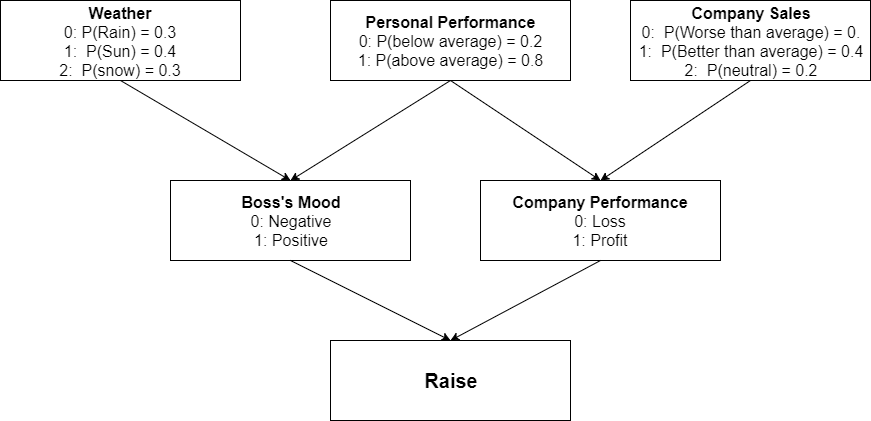
\includegraphics{images/Raise Network.png}
\caption{image}
\end{figure}

The top level variables show the prior probabilities in the node. The
other probabilities we need to specify are the conditionals for the
mid-level nodes (Boss's Mood and Profits) and the final node (Raise).
All of these variables depend on two parent variables, with the mid
level nodes having 6 entries in the conditional probability table
(representing all possible states of the parents) and the Raise node
having four entries in the conditional probability table. The tables are
presented below:

Conditional Probability of Boss's Mood

\begin{longtable}[]{@{}lll@{}}
\toprule
Weather & Personal Performance & P(Mood = Positive)\tabularnewline
\midrule
\endhead
0 & 0 & 0.15\tabularnewline
0 & 1 & 0.55\tabularnewline
1 & 0 & 0.45\tabularnewline
1 & 1 & 0.85\tabularnewline
2 & 0 & 0.35\tabularnewline
2 & 1 & 0.75\tabularnewline
\bottomrule
\end{longtable}

Conditional Probability of Company Performance

\begin{longtable}[]{@{}lll@{}}
\toprule
Company Revenue & Personal Performance & P(Company Performance =
Profit)\tabularnewline
\midrule
\endhead
0 & 0 & 0.05\tabularnewline
0 & 1 & 0.10\tabularnewline
1 & 0 & 0.75\tabularnewline
1 & 1 & 0.95\tabularnewline
2 & 0 & 0.20\tabularnewline
2 & 1 & 0.40\tabularnewline
\bottomrule
\end{longtable}

Conditional Probability of Raise

\begin{longtable}[]{@{}lll@{}}
\toprule
Boss's Mood & Company Performance & P(Raise = True)\tabularnewline
\midrule
\endhead
0 & 0 & 0.05\tabularnewline
0 & 1 & 0.65\tabularnewline
1 & 0 & 0.40\tabularnewline
1 & 1 & 0.90\tabularnewline
\bottomrule
\end{longtable}

With the prior probabilities and the conditional probabilities, we can
compute the entire joint probability of the network. We can also use
Markov Chain Monte Carlo to approximate the posterior probabilities of
any variables in the network with or without observations.

    \hypertarget{a.-discrete-bayesian-network-in-pymc3}{%
\subsection{A. Discrete Bayesian Network in
PyMC3}\label{a.-discrete-bayesian-network-in-pymc3}}

The first approach to solve this network uses a Markov Chain Monte Carlo
algorithm to find approximate probabilities. MCMC works by sampling from
the posterior distribution to find an approximation of the posterior and
the accuracy increases as the number of samples increases. PyMC3
implements Bayesian Reasoning by constructing a graph of the network and
then evaluating the graph during the sampling process. In this problem
we have only two kinds of variables: binary (taking on two values), and
discrete (in this case taking on 3 values). We can build up the graph
and then query it to find the approximate probabilities without and then
with evidence (observations).

    \begin{Verbatim}[commandchars=\\\{\}]
{\color{incolor}In [{\color{incolor}20}]:} \PY{k+kn}{import} \PY{n+nn}{numpy} \PY{k}{as} \PY{n+nn}{np}
         \PY{k+kn}{import} \PY{n+nn}{pandas} \PY{k}{as} \PY{n+nn}{pd}
         
         \PY{k+kn}{import} \PY{n+nn}{pymc3} \PY{k}{as} \PY{n+nn}{pm}
         
         \PY{k+kn}{import} \PY{n+nn}{matplotlib}\PY{n+nn}{.}\PY{n+nn}{pyplot} \PY{k}{as} \PY{n+nn}{plt}
         \PY{o}{\PYZpc{}}\PY{k}{matplotlib} inline
         
         \PY{k+kn}{import} \PY{n+nn}{theano}\PY{n+nn}{.}\PY{n+nn}{tensor} \PY{k}{as} \PY{n+nn}{tt}
         \PY{k+kn}{import} \PY{n+nn}{matplotlib}
         
         \PY{k+kn}{import} \PY{n+nn}{seaborn} \PY{k}{as} \PY{n+nn}{sns}
         
         \PY{k+kn}{from} \PY{n+nn}{IPython}\PY{n+nn}{.}\PY{n+nn}{core}\PY{n+nn}{.}\PY{n+nn}{pylabtools} \PY{k}{import} \PY{n}{figsize}
\end{Verbatim}


    \hypertarget{construct-the-model-graph}{%
\subsubsection{Construct the Model
Graph}\label{construct-the-model-graph}}

First, we make the network in pymc3. We specify the prior probabilities
and the conditional probability tables. In pymc3, the conditional
probabilities are represented using switch statements.

    \begin{Verbatim}[commandchars=\\\{\}]
{\color{incolor}In [{\color{incolor}3}]:} \PY{n}{N\PYZus{}SAMPLES} \PY{o}{=} \PY{l+m+mi}{1000}
        \PY{n}{N\PYZus{}CHAINS} \PY{o}{=} \PY{l+m+mi}{2}
        
        \PY{k}{with} \PY{n}{pm}\PY{o}{.}\PY{n}{Model}\PY{p}{(}\PY{p}{)} \PY{k}{as} \PY{n}{raise\PYZus{}model}\PY{p}{:}
            
            \PY{c+c1}{\PYZsh{} Weather is a categorical variable with 3 states}
            \PY{n}{weather} \PY{o}{=} \PY{n}{pm}\PY{o}{.}\PY{n}{Categorical}\PY{p}{(}\PY{l+s+s1}{\PYZsq{}}\PY{l+s+s1}{weather}\PY{l+s+s1}{\PYZsq{}}\PY{p}{,} \PY{n}{np}\PY{o}{.}\PY{n}{array}\PY{p}{(}\PY{p}{[}\PY{l+m+mf}{0.3}\PY{p}{,} \PY{l+m+mf}{0.4}\PY{p}{,} \PY{l+m+mf}{0.3}\PY{p}{]}\PY{p}{)}\PY{p}{)}
            
            \PY{c+c1}{\PYZsh{} Personal Performance is a Bernoulli Variable with 2 states}
            \PY{n}{pp} \PY{o}{=} \PY{n}{pm}\PY{o}{.}\PY{n}{Bernoulli}\PY{p}{(}\PY{l+s+s1}{\PYZsq{}}\PY{l+s+s1}{pp}\PY{l+s+s1}{\PYZsq{}}\PY{p}{,} \PY{l+m+mf}{0.8}\PY{p}{)}
            
            \PY{c+c1}{\PYZsh{} Company Revenue is a categorical variable with 3 states}
            \PY{n}{revenue} \PY{o}{=} \PY{n}{pm}\PY{o}{.}\PY{n}{Categorical}\PY{p}{(}\PY{l+s+s1}{\PYZsq{}}\PY{l+s+s1}{revenue}\PY{l+s+s1}{\PYZsq{}}\PY{p}{,} \PY{n}{np}\PY{o}{.}\PY{n}{array}\PY{p}{(}\PY{p}{[}\PY{l+m+mf}{0.4}\PY{p}{,} \PY{l+m+mf}{0.4}\PY{p}{,} \PY{l+m+mf}{0.2}\PY{p}{]}\PY{p}{)}\PY{p}{)}
            
            \PY{c+c1}{\PYZsh{} Boss\PYZsq{}s Mood Conditional Probability Definition}
            \PY{n}{mood} \PY{o}{=} \PY{n}{pm}\PY{o}{.}\PY{n}{Bernoulli}\PY{p}{(}\PY{l+s+s1}{\PYZsq{}}\PY{l+s+s1}{mood}\PY{l+s+s1}{\PYZsq{}}\PY{p}{,} \PY{n}{tt}\PY{o}{.}\PY{n}{switch}\PY{p}{(}\PY{n}{tt}\PY{o}{.}\PY{n}{eq}\PY{p}{(}\PY{n}{weather}\PY{p}{,} \PY{l+m+mi}{0}\PY{p}{)}\PY{p}{,} \PY{n}{tt}\PY{o}{.}\PY{n}{switch}\PY{p}{(}\PY{n}{tt}\PY{o}{.}\PY{n}{eq}\PY{p}{(}\PY{n}{pp}\PY{p}{,} \PY{l+m+mi}{0}\PY{p}{)}\PY{p}{,} \PY{l+m+mf}{0.15}\PY{p}{,} \PY{l+m+mf}{0.55}\PY{p}{)}\PY{p}{,} 
                                                  \PY{n}{tt}\PY{o}{.}\PY{n}{switch}\PY{p}{(}\PY{n}{tt}\PY{o}{.}\PY{n}{eq}\PY{p}{(}\PY{n}{weather}\PY{p}{,} \PY{l+m+mi}{1}\PY{p}{)}\PY{p}{,} \PY{n}{tt}\PY{o}{.}\PY{n}{switch}\PY{p}{(}\PY{n}{tt}\PY{o}{.}\PY{n}{eq}\PY{p}{(}\PY{n}{pp}\PY{p}{,} \PY{l+m+mi}{0}\PY{p}{)}\PY{p}{,} \PY{l+m+mf}{0.45}\PY{p}{,} \PY{l+m+mf}{0.85}\PY{p}{)}\PY{p}{,} 
                                                                               \PY{n}{tt}\PY{o}{.}\PY{n}{switch}\PY{p}{(}\PY{n}{tt}\PY{o}{.}\PY{n}{eq}\PY{p}{(}\PY{n}{pp}\PY{p}{,} \PY{l+m+mi}{0}\PY{p}{)}\PY{p}{,} \PY{l+m+mf}{0.35}\PY{p}{,} \PY{l+m+mf}{0.75}\PY{p}{)}\PY{p}{)}\PY{p}{)}\PY{p}{)}
            
            \PY{c+c1}{\PYZsh{} Company Performance Conditional Probability Definition}
            \PY{n}{cp} \PY{o}{=} \PY{n}{pm}\PY{o}{.}\PY{n}{Bernoulli}\PY{p}{(}\PY{l+s+s1}{\PYZsq{}}\PY{l+s+s1}{cp}\PY{l+s+s1}{\PYZsq{}}\PY{p}{,} \PY{n}{tt}\PY{o}{.}\PY{n}{switch}\PY{p}{(}\PY{n}{tt}\PY{o}{.}\PY{n}{eq}\PY{p}{(}\PY{n}{revenue}\PY{p}{,} \PY{l+m+mi}{0}\PY{p}{)}\PY{p}{,} \PY{n}{tt}\PY{o}{.}\PY{n}{switch}\PY{p}{(}\PY{n}{tt}\PY{o}{.}\PY{n}{eq}\PY{p}{(}\PY{n}{pp}\PY{p}{,} \PY{l+m+mi}{0}\PY{p}{)}\PY{p}{,} \PY{l+m+mf}{0.05}\PY{p}{,} \PY{l+m+mf}{0.10}\PY{p}{)}\PY{p}{,}
                                              \PY{n}{tt}\PY{o}{.}\PY{n}{switch}\PY{p}{(}\PY{n}{tt}\PY{o}{.}\PY{n}{eq}\PY{p}{(}\PY{n}{revenue}\PY{p}{,} \PY{l+m+mi}{1}\PY{p}{)}\PY{p}{,} \PY{n}{tt}\PY{o}{.}\PY{n}{switch}\PY{p}{(}\PY{n}{tt}\PY{o}{.}\PY{n}{eq}\PY{p}{(}\PY{n}{pp}\PY{p}{,} \PY{l+m+mi}{0}\PY{p}{)}\PY{p}{,} \PY{l+m+mf}{0.75}\PY{p}{,} \PY{l+m+mf}{0.95}\PY{p}{)}\PY{p}{,}
                                                                    \PY{n}{tt}\PY{o}{.}\PY{n}{switch}\PY{p}{(}\PY{n}{tt}\PY{o}{.}\PY{n}{eq}\PY{p}{(}\PY{n}{pp}\PY{p}{,} \PY{l+m+mi}{0}\PY{p}{)}\PY{p}{,} \PY{l+m+mf}{0.20}\PY{p}{,} \PY{l+m+mf}{0.40}\PY{p}{)}\PY{p}{)}\PY{p}{)}\PY{p}{)}
            
            \PY{c+c1}{\PYZsh{} Raise is a Bernoulli Variable with 2 states}
            \PY{n}{raise\PYZus{}} \PY{o}{=} \PY{n}{pm}\PY{o}{.}\PY{n}{Bernoulli}\PY{p}{(}\PY{l+s+s1}{\PYZsq{}}\PY{l+s+s1}{raise\PYZus{}}\PY{l+s+s1}{\PYZsq{}}\PY{p}{,} \PY{n}{tt}\PY{o}{.}\PY{n}{switch}\PY{p}{(}\PY{n}{tt}\PY{o}{.}\PY{n}{eq}\PY{p}{(}\PY{n}{mood}\PY{p}{,} \PY{l+m+mi}{0}\PY{p}{)}\PY{p}{,} \PY{n}{tt}\PY{o}{.}\PY{n}{switch}\PY{p}{(}\PY{n}{tt}\PY{o}{.}\PY{n}{eq}\PY{p}{(}\PY{n}{cp}\PY{p}{,} \PY{l+m+mi}{0}\PY{p}{)}\PY{p}{,} \PY{l+m+mf}{0.05}\PY{p}{,} \PY{l+m+mf}{0.65}\PY{p}{)}\PY{p}{,}
                                                                      \PY{n}{tt}\PY{o}{.}\PY{n}{switch}\PY{p}{(}\PY{n}{tt}\PY{o}{.}\PY{n}{eq}\PY{p}{(}\PY{n}{cp}\PY{p}{,} \PY{l+m+mi}{0}\PY{p}{)}\PY{p}{,} \PY{l+m+mf}{0.40}\PY{p}{,} \PY{l+m+mf}{0.90}\PY{p}{)}\PY{p}{)}\PY{p}{)}
                                         
\end{Verbatim}


    \hypertarget{sample-from-the-posterior-using-the-gibbs-metropolis-algorithm}{%
\subsubsection{Sample from the Posterior Using the Gibbs Metropolis
Algorithm}\label{sample-from-the-posterior-using-the-gibbs-metropolis-algorithm}}

After the graph is built, we can draw samples from the posterior
distribution using a Markov Chain Monte Carlo approach called Gibbs
Metropolis. At each step, the algorithm draws a new sample from the
posterior based on the provided probabilities. This is a Markov Chain
because the next state depends only a bounded subset of past states.
MCMC can be compared to a random walk: from a given state, there are a
limited number of random steps available to move. In this case, we are
sampling with no observations, but if we have observations, we can
compare the samples to the observations using rejection sampling. If the
sample does not agree with the evidence, it is rejected, otherwise, the
sample is accepted and becomes the current state. The model converges as
the number of steps increases.

    \begin{Verbatim}[commandchars=\\\{\}]
{\color{incolor}In [{\color{incolor}4}]:} \PY{k}{with} \PY{n}{raise\PYZus{}model}\PY{p}{:}
            \PY{c+c1}{\PYZsh{} Sample and plot traces}
            \PY{n}{raise\PYZus{}trace} \PY{o}{=} \PY{n}{pm}\PY{o}{.}\PY{n}{sample}\PY{p}{(}\PY{n}{draws}\PY{o}{=}\PY{n}{N\PYZus{}SAMPLES}\PY{p}{,} \PY{n}{chains}\PY{o}{=}\PY{n}{N\PYZus{}CHAINS}\PY{p}{)}
            \PY{n}{pm}\PY{o}{.}\PY{n}{traceplot}\PY{p}{(}\PY{n}{raise\PYZus{}trace}\PY{p}{)}
\end{Verbatim}


    \begin{Verbatim}[commandchars=\\\{\}]
Multiprocess sampling (2 chains in 2 jobs)
CompoundStep
>CategoricalGibbsMetropolis: [revenue, weather]
>BinaryGibbsMetropolis: [pp, mood, cp, raise\_]

    \end{Verbatim}

    \begin{center}
    \adjustimage{max size={0.9\linewidth}{0.9\paperheight}}{output_7_1.png}
    \end{center}
    { \hspace*{\fill} \\}
    
    \hypertarget{evaluate-the-trace-to-find-probabilities}{%
\subsection{Evaluate the Trace to Find
Probabilities}\label{evaluate-the-trace-to-find-probabilities}}

Using the sample trace, we can find the probability of different nodes
in the network. In this case, we are taking the mean of the trace
variables to represent the most likely value for a parameter.

    \begin{Verbatim}[commandchars=\\\{\}]
{\color{incolor}In [{\color{incolor}5}]:} \PY{k}{def} \PY{n+nf}{query\PYZus{}model}\PY{p}{(}\PY{n}{trace}\PY{p}{,} \PY{n}{obs}\PY{o}{=}\PY{p}{\PYZob{}}\PY{p}{\PYZcb{}}\PY{p}{,} \PY{n}{compare}\PY{o}{=}\PY{k+kc}{False}\PY{p}{)}\PY{p}{:}
            \PY{k}{if} \PY{l+s+s1}{\PYZsq{}}\PY{l+s+s1}{weather}\PY{l+s+s1}{\PYZsq{}} \PY{o+ow}{in} \PY{n}{obs}\PY{o}{.}\PY{n}{keys}\PY{p}{(}\PY{p}{)}\PY{p}{:}
                \PY{n}{f\PYZus{}rain} \PY{o}{=} \PY{n}{obs}\PY{p}{[}\PY{l+s+s1}{\PYZsq{}}\PY{l+s+s1}{weather}\PY{l+s+s1}{\PYZsq{}}\PY{p}{]}\PY{o}{.}\PY{n}{get}\PY{p}{(}\PY{l+s+s1}{\PYZsq{}}\PY{l+s+s1}{rain}\PY{l+s+s1}{\PYZsq{}}\PY{p}{,} \PY{l+m+mi}{0}\PY{p}{)}
                \PY{n}{f\PYZus{}sun} \PY{o}{=} \PY{n}{obs}\PY{p}{[}\PY{l+s+s1}{\PYZsq{}}\PY{l+s+s1}{weather}\PY{l+s+s1}{\PYZsq{}}\PY{p}{]}\PY{o}{.}\PY{n}{get}\PY{p}{(}\PY{l+s+s1}{\PYZsq{}}\PY{l+s+s1}{sun}\PY{l+s+s1}{\PYZsq{}}\PY{p}{,} \PY{l+m+mi}{0}\PY{p}{)}
                \PY{n}{f\PYZus{}snow} \PY{o}{=} \PY{n}{obs}\PY{p}{[}\PY{l+s+s1}{\PYZsq{}}\PY{l+s+s1}{weather}\PY{l+s+s1}{\PYZsq{}}\PY{p}{]}\PY{o}{.}\PY{n}{get}\PY{p}{(}\PY{l+s+s1}{\PYZsq{}}\PY{l+s+s1}{snow}\PY{l+s+s1}{\PYZsq{}}\PY{p}{,} \PY{l+m+mi}{0}\PY{p}{)}
                
            \PY{k}{else}\PY{p}{:}
                \PY{n}{f\PYZus{}rain} \PY{o}{=} \PY{n}{np}\PY{o}{.}\PY{n}{mean}\PY{p}{(}\PY{n}{trace}\PY{p}{[}\PY{l+s+s1}{\PYZsq{}}\PY{l+s+s1}{weather}\PY{l+s+s1}{\PYZsq{}}\PY{p}{]} \PY{o}{\PYZlt{}} \PY{l+m+mf}{0.5}\PY{p}{)}
                \PY{n}{f\PYZus{}sun} \PY{o}{=} \PY{n}{np}\PY{o}{.}\PY{n}{mean}\PY{p}{(}\PY{p}{(}\PY{n}{trace}\PY{p}{[}\PY{l+s+s1}{\PYZsq{}}\PY{l+s+s1}{weather}\PY{l+s+s1}{\PYZsq{}}\PY{p}{]} \PY{o}{\PYZgt{}}\PY{o}{=} \PY{l+m+mf}{0.5}\PY{p}{)} \PY{o}{\PYZam{}} \PY{p}{(}\PY{n}{trace}\PY{p}{[}\PY{l+s+s1}{\PYZsq{}}\PY{l+s+s1}{weather}\PY{l+s+s1}{\PYZsq{}}\PY{p}{]} \PY{o}{\PYZlt{}}\PY{o}{=} \PY{l+m+mf}{1.5}\PY{p}{)}\PY{p}{)}
                \PY{n}{f\PYZus{}snow} \PY{o}{=} \PY{n}{np}\PY{o}{.}\PY{n}{mean}\PY{p}{(}\PY{n}{trace}\PY{p}{[}\PY{l+s+s1}{\PYZsq{}}\PY{l+s+s1}{weather}\PY{l+s+s1}{\PYZsq{}}\PY{p}{]} \PY{o}{\PYZgt{}} \PY{l+m+mf}{1.5}\PY{p}{)}
            
            \PY{n+nb}{print}\PY{p}{(}\PY{l+s+s1}{\PYZsq{}}\PY{l+s+s1}{Approximate Probabilities from MCMC:}\PY{l+s+s1}{\PYZsq{}}\PY{p}{)}
            \PY{n+nb}{print}\PY{p}{(}\PY{l+s+s2}{\PYZdq{}\PYZdq{}\PYZdq{}}\PY{l+s+se}{\PYZbs{}n}\PY{l+s+s2}{Weather: }\PY{l+s+si}{\PYZob{}:.2f\PYZcb{}}\PY{l+s+s2}{, }\PY{l+s+si}{\PYZob{}:.2f\PYZcb{}}\PY{l+s+s2}{, }\PY{l+s+si}{\PYZob{}:.2f\PYZcb{}}\PY{l+s+s2}{.}\PY{l+s+s2}{\PYZdq{}\PYZdq{}\PYZdq{}}\PY{o}{.}\PY{n}{format}\PY{p}{(}
                      \PY{n}{f\PYZus{}rain}\PY{p}{,} \PY{n}{f\PYZus{}sun}\PY{p}{,} \PY{n}{f\PYZus{}snow}\PY{p}{)}\PY{p}{)}
            
            \PY{k}{if} \PY{l+s+s1}{\PYZsq{}}\PY{l+s+s1}{pp}\PY{l+s+s1}{\PYZsq{}} \PY{o+ow}{in} \PY{n}{obs}\PY{o}{.}\PY{n}{keys}\PY{p}{(}\PY{p}{)}\PY{p}{:}
                \PY{n}{f\PYZus{}pp\PYZus{}above} \PY{o}{=} \PY{n}{obs}\PY{p}{[}\PY{l+s+s1}{\PYZsq{}}\PY{l+s+s1}{pp}\PY{l+s+s1}{\PYZsq{}}\PY{p}{]}\PY{o}{.}\PY{n}{get}\PY{p}{(}\PY{l+s+s1}{\PYZsq{}}\PY{l+s+s1}{pp}\PY{l+s+s1}{\PYZsq{}}\PY{p}{)}
            
            \PY{k}{else}\PY{p}{:}
                \PY{n}{f\PYZus{}pp\PYZus{}above} \PY{o}{=} \PY{n}{np}\PY{o}{.}\PY{n}{mean}\PY{p}{(}\PY{n}{trace}\PY{p}{[}\PY{l+s+s1}{\PYZsq{}}\PY{l+s+s1}{pp}\PY{l+s+s1}{\PYZsq{}}\PY{p}{]} \PY{o}{\PYZgt{}}\PY{o}{=} \PY{l+m+mf}{0.5}\PY{p}{)}
                
            \PY{n}{f\PYZus{}pp\PYZus{}below} \PY{o}{=} \PY{l+m+mi}{1} \PY{o}{\PYZhy{}} \PY{n}{f\PYZus{}pp\PYZus{}above}
            \PY{n+nb}{print}\PY{p}{(}\PY{l+s+s2}{\PYZdq{}\PYZdq{}\PYZdq{}}\PY{l+s+s2}{Personal Performance: }\PY{l+s+si}{\PYZob{}:.2f\PYZcb{}}\PY{l+s+s2}{, }\PY{l+s+si}{\PYZob{}:.2f\PYZcb{}}\PY{l+s+s2}{\PYZdq{}\PYZdq{}\PYZdq{}}\PY{o}{.}\PY{n}{format}\PY{p}{(}
                     \PY{n}{f\PYZus{}pp\PYZus{}below}\PY{p}{,} \PY{n}{f\PYZus{}pp\PYZus{}above}\PY{p}{)}\PY{p}{)}
            
            \PY{k}{if} \PY{l+s+s1}{\PYZsq{}}\PY{l+s+s1}{revenue}\PY{l+s+s1}{\PYZsq{}} \PY{o+ow}{in} \PY{n}{obs}\PY{o}{.}\PY{n}{keys}\PY{p}{(}\PY{p}{)}\PY{p}{:}
                \PY{n}{f\PYZus{}revenue\PYZus{}below} \PY{o}{=} \PY{n}{obs}\PY{p}{[}\PY{l+s+s1}{\PYZsq{}}\PY{l+s+s1}{revenue}\PY{l+s+s1}{\PYZsq{}}\PY{p}{]}\PY{o}{.}\PY{n}{get}\PY{p}{(}\PY{l+s+s1}{\PYZsq{}}\PY{l+s+s1}{below}\PY{l+s+s1}{\PYZsq{}}\PY{p}{,} \PY{l+m+mi}{0}\PY{p}{)}
                \PY{n}{f\PYZus{}revenue\PYZus{}above} \PY{o}{=} \PY{n}{obs}\PY{p}{[}\PY{l+s+s1}{\PYZsq{}}\PY{l+s+s1}{revenue}\PY{l+s+s1}{\PYZsq{}}\PY{p}{]}\PY{o}{.}\PY{n}{get}\PY{p}{(}\PY{l+s+s1}{\PYZsq{}}\PY{l+s+s1}{above}\PY{l+s+s1}{\PYZsq{}}\PY{p}{,} \PY{l+m+mi}{0}\PY{p}{)}
                \PY{n}{f\PYZus{}revenue\PYZus{}neutral} \PY{o}{=} \PY{n}{obs}\PY{p}{[}\PY{l+s+s1}{\PYZsq{}}\PY{l+s+s1}{revenue}\PY{l+s+s1}{\PYZsq{}}\PY{p}{]}\PY{o}{.}\PY{n}{get}\PY{p}{(}\PY{l+s+s1}{\PYZsq{}}\PY{l+s+s1}{neutral}\PY{l+s+s1}{\PYZsq{}}\PY{p}{,} \PY{l+m+mi}{0}\PY{p}{)}
                
            \PY{k}{else}\PY{p}{:}
                \PY{n}{f\PYZus{}revenue\PYZus{}below} \PY{o}{=} \PY{n}{np}\PY{o}{.}\PY{n}{mean}\PY{p}{(}\PY{n}{trace}\PY{p}{[}\PY{l+s+s1}{\PYZsq{}}\PY{l+s+s1}{revenue}\PY{l+s+s1}{\PYZsq{}}\PY{p}{]} \PY{o}{\PYZlt{}} \PY{l+m+mf}{0.5}\PY{p}{)}
                \PY{n}{f\PYZus{}revenue\PYZus{}above} \PY{o}{=} \PY{n}{np}\PY{o}{.}\PY{n}{mean}\PY{p}{(}\PY{p}{(}\PY{n}{trace}\PY{p}{[}\PY{l+s+s1}{\PYZsq{}}\PY{l+s+s1}{revenue}\PY{l+s+s1}{\PYZsq{}}\PY{p}{]} \PY{o}{\PYZgt{}}\PY{o}{=} \PY{l+m+mf}{0.5}\PY{p}{)} \PY{o}{\PYZam{}} \PY{p}{(}\PY{n}{trace}\PY{p}{[}\PY{l+s+s1}{\PYZsq{}}\PY{l+s+s1}{revenue}\PY{l+s+s1}{\PYZsq{}}\PY{p}{]} \PY{o}{\PYZlt{}}\PY{o}{=} \PY{l+m+mf}{1.5}\PY{p}{)}\PY{p}{)}
                \PY{n}{f\PYZus{}revenue\PYZus{}neutral} \PY{o}{=} \PY{n}{np}\PY{o}{.}\PY{n}{mean}\PY{p}{(}\PY{n}{trace}\PY{p}{[}\PY{l+s+s1}{\PYZsq{}}\PY{l+s+s1}{revenue}\PY{l+s+s1}{\PYZsq{}}\PY{p}{]} \PY{o}{\PYZgt{}} \PY{l+m+mf}{1.5}\PY{p}{)}
            \PY{n+nb}{print}\PY{p}{(}\PY{l+s+s2}{\PYZdq{}\PYZdq{}\PYZdq{}}\PY{l+s+s2}{Revenue: }\PY{l+s+si}{\PYZob{}:.2f\PYZcb{}}\PY{l+s+s2}{, }\PY{l+s+si}{\PYZob{}:.2f\PYZcb{}}\PY{l+s+s2}{, }\PY{l+s+si}{\PYZob{}:.2f\PYZcb{}}\PY{l+s+s2}{.}\PY{l+s+s2}{\PYZdq{}\PYZdq{}\PYZdq{}}\PY{o}{.}\PY{n}{format}\PY{p}{(}
                      \PY{n}{f\PYZus{}revenue\PYZus{}below}\PY{p}{,} \PY{n}{f\PYZus{}revenue\PYZus{}above}\PY{p}{,} \PY{n}{f\PYZus{}revenue\PYZus{}neutral}\PY{p}{)}\PY{p}{)}
            
            \PY{k}{if} \PY{l+s+s1}{\PYZsq{}}\PY{l+s+s1}{mood}\PY{l+s+s1}{\PYZsq{}} \PY{o+ow}{in} \PY{n}{obs}\PY{o}{.}\PY{n}{keys}\PY{p}{(}\PY{p}{)}\PY{p}{:}
                \PY{n}{f\PYZus{}mood\PYZus{}positive} \PY{o}{=} \PY{n}{obs}\PY{p}{[}\PY{l+s+s1}{\PYZsq{}}\PY{l+s+s1}{mood}\PY{l+s+s1}{\PYZsq{}}\PY{p}{]}\PY{o}{.}\PY{n}{get}\PY{p}{(}\PY{l+s+s1}{\PYZsq{}}\PY{l+s+s1}{mood}\PY{l+s+s1}{\PYZsq{}}\PY{p}{)}
            \PY{k}{else}\PY{p}{:}
                \PY{n}{f\PYZus{}mood\PYZus{}positive} \PY{o}{=} \PY{n}{np}\PY{o}{.}\PY{n}{mean}\PY{p}{(}\PY{n}{trace}\PY{p}{[}\PY{l+s+s1}{\PYZsq{}}\PY{l+s+s1}{mood}\PY{l+s+s1}{\PYZsq{}}\PY{p}{]} \PY{o}{\PYZgt{}}\PY{o}{=} \PY{l+m+mf}{0.5}\PY{p}{)}
            
            \PY{n}{f\PYZus{}mood\PYZus{}negative} \PY{o}{=} \PY{l+m+mi}{1} \PY{o}{\PYZhy{}} \PY{n}{f\PYZus{}mood\PYZus{}positive}
            \PY{n+nb}{print}\PY{p}{(}\PY{l+s+s2}{\PYZdq{}\PYZdq{}\PYZdq{}}\PY{l+s+s2}{Boss}\PY{l+s+s2}{\PYZsq{}}\PY{l+s+s2}{s mood: }\PY{l+s+si}{\PYZob{}:.2f\PYZcb{}}\PY{l+s+s2}{, }\PY{l+s+si}{\PYZob{}:.2f\PYZcb{}}\PY{l+s+s2}{.}\PY{l+s+s2}{\PYZdq{}\PYZdq{}\PYZdq{}}\PY{o}{.}\PY{n}{format}\PY{p}{(}
                \PY{n}{f\PYZus{}mood\PYZus{}negative}\PY{p}{,} \PY{n}{f\PYZus{}mood\PYZus{}positive}\PY{p}{)}\PY{p}{)}
            
            \PY{k}{if} \PY{l+s+s1}{\PYZsq{}}\PY{l+s+s1}{cp}\PY{l+s+s1}{\PYZsq{}} \PY{o+ow}{in} \PY{n}{obs}\PY{o}{.}\PY{n}{keys}\PY{p}{(}\PY{p}{)}\PY{p}{:}
                \PY{n}{f\PYZus{}profits} \PY{o}{=} \PY{n}{obs}\PY{p}{[}\PY{l+s+s1}{\PYZsq{}}\PY{l+s+s1}{cp}\PY{l+s+s1}{\PYZsq{}}\PY{p}{]}\PY{o}{.}\PY{n}{get}\PY{p}{(}\PY{l+s+s1}{\PYZsq{}}\PY{l+s+s1}{cp}\PY{l+s+s1}{\PYZsq{}}\PY{p}{)}
            \PY{k}{else}\PY{p}{:}
                \PY{n}{f\PYZus{}profits} \PY{o}{=} \PY{n}{np}\PY{o}{.}\PY{n}{mean}\PY{p}{(}\PY{n}{trace}\PY{p}{[}\PY{l+s+s1}{\PYZsq{}}\PY{l+s+s1}{cp}\PY{l+s+s1}{\PYZsq{}}\PY{p}{]} \PY{o}{\PYZgt{}}\PY{o}{=} \PY{l+m+mf}{0.5}\PY{p}{)}
            
            \PY{n}{f\PYZus{}loss} \PY{o}{=} \PY{l+m+mi}{1} \PY{o}{\PYZhy{}} \PY{n}{f\PYZus{}profits}
            
            \PY{n+nb}{print}\PY{p}{(}\PY{l+s+s2}{\PYZdq{}\PYZdq{}\PYZdq{}}\PY{l+s+s2}{Profits: }\PY{l+s+si}{\PYZob{}:.2f\PYZcb{}}\PY{l+s+s2}{, }\PY{l+s+si}{\PYZob{}:.2f\PYZcb{}}\PY{l+s+s2}{.}\PY{l+s+s2}{\PYZdq{}\PYZdq{}\PYZdq{}}\PY{o}{.}\PY{n}{format}\PY{p}{(}
                \PY{n}{f\PYZus{}loss}\PY{p}{,} \PY{n}{f\PYZus{}profits}\PY{p}{)}\PY{p}{)}
            
            \PY{k}{if} \PY{l+s+s1}{\PYZsq{}}\PY{l+s+s1}{raise}\PY{l+s+s1}{\PYZsq{}} \PY{o+ow}{in} \PY{n}{obs}\PY{o}{.}\PY{n}{keys}\PY{p}{(}\PY{p}{)}\PY{p}{:}
                \PY{n}{f\PYZus{}raise} \PY{o}{=} \PY{n}{obs}\PY{p}{[}\PY{l+s+s1}{\PYZsq{}}\PY{l+s+s1}{raise}\PY{l+s+s1}{\PYZsq{}}\PY{p}{]}\PY{o}{.}\PY{n}{get}\PY{p}{(}\PY{l+s+s1}{\PYZsq{}}\PY{l+s+s1}{raise}\PY{l+s+s1}{\PYZsq{}}\PY{p}{)}
                
            \PY{k}{else}\PY{p}{:}
                \PY{n}{f\PYZus{}raise} \PY{o}{=} \PY{n}{np}\PY{o}{.}\PY{n}{mean}\PY{p}{(}\PY{n}{trace}\PY{p}{[}\PY{l+s+s1}{\PYZsq{}}\PY{l+s+s1}{raise\PYZus{}}\PY{l+s+s1}{\PYZsq{}}\PY{p}{]} \PY{o}{\PYZgt{}}\PY{o}{=} \PY{l+m+mf}{0.5}\PY{p}{)}
            
            \PY{n+nb}{print}\PY{p}{(}\PY{l+s+s2}{\PYZdq{}\PYZdq{}\PYZdq{}}\PY{l+s+se}{\PYZbs{}n}\PY{l+s+s2}{Probability of a raise: }\PY{l+s+si}{\PYZob{}:.4f\PYZcb{}}\PY{l+s+s2}{.}\PY{l+s+s2}{\PYZdq{}\PYZdq{}\PYZdq{}}\PY{o}{.}\PY{n}{format}\PY{p}{(}\PY{n}{f\PYZus{}raise}\PY{p}{)}\PY{p}{)}
            
            \PY{k}{if} \PY{n}{compare}\PY{p}{:}
                \PY{k}{return} \PY{p}{[}\PY{n}{f\PYZus{}rain}\PY{p}{,} \PY{n}{f\PYZus{}sun}\PY{p}{,} \PY{n}{f\PYZus{}snow}\PY{p}{,} \PY{n}{f\PYZus{}pp\PYZus{}above}\PY{p}{,} \PY{n}{f\PYZus{}revenue\PYZus{}below}\PY{p}{,} 
                        \PY{n}{f\PYZus{}revenue\PYZus{}above}\PY{p}{,} \PY{n}{f\PYZus{}revenue\PYZus{}neutral}\PY{p}{,} \PY{n}{f\PYZus{}mood\PYZus{}positive}\PY{p}{,}
                        \PY{n}{f\PYZus{}profits}\PY{p}{,} \PY{n}{f\PYZus{}raise}\PY{p}{]}
\end{Verbatim}


    \hypertarget{approximate-probabilities-with-no-evidence}{%
\subsubsection{Approximate Probabilities with No
Evidence}\label{approximate-probabilities-with-no-evidence}}

The first query we will make finds the approximate probability of a
raise with no evidence.

    \begin{Verbatim}[commandchars=\\\{\}]
{\color{incolor}In [{\color{incolor}6}]:} \PY{n}{query\PYZus{}model}\PY{p}{(}\PY{n}{raise\PYZus{}trace}\PY{p}{)}
\end{Verbatim}


    \begin{Verbatim}[commandchars=\\\{\}]
Approximate Probabilities from MCMC:

Weather: 0.30, 0.40, 0.30.
Personal Performance: 0.21, 0.79
Revenue: 0.39, 0.40, 0.21.
Boss's mood: 0.36, 0.64.
Profits: 0.54, 0.46.

Probability of a raise: 0.5140.

    \end{Verbatim}

    We can see based only on the priors and conditional probabilities, with
no observations, there is a slightly over 50\% chance of a raise.

    \hypertarget{model-accounting-for-observations}{%
\subsection{Model Accounting for
Observations}\label{model-accounting-for-observations}}

If we do have observations, such as the weather, personal performance,
or revenue, we can feed those into the model to update our estimate.
This is the essence of Bayesian Inference: we have prior beliefs, that
we subsequently update as we gather more information. Bayes Rule is
expressed below:

\[ P(A|B) = \frac{P(B|A) * P(A)}{P(B)} = \frac{\text{likelihoood} * \text{prior}}{\text{normalization}}\]

    \begin{Verbatim}[commandchars=\\\{\}]
{\color{incolor}In [{\color{incolor}7}]:} \PY{k}{def} \PY{n+nf}{model\PYZus{}with\PYZus{}evidence}\PY{p}{(}\PY{n}{weather\PYZus{}obs}\PY{o}{=}\PY{k+kc}{None}\PY{p}{,} \PY{n}{pp\PYZus{}obs}\PY{o}{=}\PY{k+kc}{None}\PY{p}{,} \PY{n}{revenue\PYZus{}obs}\PY{o}{=}\PY{k+kc}{None}\PY{p}{,}
                                \PY{n}{mood\PYZus{}obs}\PY{o}{=}\PY{k+kc}{None}\PY{p}{,} \PY{n}{cp\PYZus{}obs}\PY{o}{=}\PY{k+kc}{None}\PY{p}{,} \PY{n}{raise\PYZus{}obs}\PY{o}{=}\PY{k+kc}{None}\PY{p}{)}\PY{p}{:}
            
            \PY{k}{with} \PY{n}{pm}\PY{o}{.}\PY{n}{Model}\PY{p}{(}\PY{p}{)} \PY{k}{as} \PY{n}{raise\PYZus{}model}\PY{p}{:}
            
                \PY{c+c1}{\PYZsh{} Weather is a categorical variable with 3 states}
                \PY{n}{weather} \PY{o}{=} \PY{n}{pm}\PY{o}{.}\PY{n}{Categorical}\PY{p}{(}\PY{l+s+s1}{\PYZsq{}}\PY{l+s+s1}{weather}\PY{l+s+s1}{\PYZsq{}}\PY{p}{,} \PY{n}{np}\PY{o}{.}\PY{n}{array}\PY{p}{(}\PY{p}{[}\PY{l+m+mf}{0.3}\PY{p}{,} \PY{l+m+mf}{0.4}\PY{p}{,} \PY{l+m+mf}{0.3}\PY{p}{]}\PY{p}{)}\PY{p}{,} 
                                         \PY{n}{observed} \PY{o}{=} \PY{n}{weather\PYZus{}obs}\PY{p}{)}
        
                \PY{c+c1}{\PYZsh{} Personal Performance is a Bernoulli Variable with 2 states}
                \PY{n}{pp} \PY{o}{=} \PY{n}{pm}\PY{o}{.}\PY{n}{Bernoulli}\PY{p}{(}\PY{l+s+s1}{\PYZsq{}}\PY{l+s+s1}{pp}\PY{l+s+s1}{\PYZsq{}}\PY{p}{,} \PY{l+m+mf}{0.8}\PY{p}{,} \PY{n}{observed} \PY{o}{=} \PY{n}{pp\PYZus{}obs}\PY{p}{)}
        
                \PY{c+c1}{\PYZsh{} Company Revenue is a categorical variable with 3 states}
                \PY{n}{revenue} \PY{o}{=} \PY{n}{pm}\PY{o}{.}\PY{n}{Categorical}\PY{p}{(}\PY{l+s+s1}{\PYZsq{}}\PY{l+s+s1}{revenue}\PY{l+s+s1}{\PYZsq{}}\PY{p}{,} \PY{n}{np}\PY{o}{.}\PY{n}{array}\PY{p}{(}\PY{p}{[}\PY{l+m+mf}{0.4}\PY{p}{,} \PY{l+m+mf}{0.4}\PY{p}{,} \PY{l+m+mf}{0.2}\PY{p}{]}\PY{p}{)}\PY{p}{,} 
                                         \PY{n}{observed} \PY{o}{=} \PY{n}{revenue\PYZus{}obs}\PY{p}{)}
        
                \PY{c+c1}{\PYZsh{} Boss\PYZsq{}s Mood Conditional Probability Definition}
                \PY{n}{mood} \PY{o}{=} \PY{n}{pm}\PY{o}{.}\PY{n}{Bernoulli}\PY{p}{(}\PY{l+s+s1}{\PYZsq{}}\PY{l+s+s1}{mood}\PY{l+s+s1}{\PYZsq{}}\PY{p}{,} \PY{n}{tt}\PY{o}{.}\PY{n}{switch}\PY{p}{(}\PY{n}{tt}\PY{o}{.}\PY{n}{eq}\PY{p}{(}\PY{n}{weather}\PY{p}{,} \PY{l+m+mi}{0}\PY{p}{)}\PY{p}{,} \PY{n}{tt}\PY{o}{.}\PY{n}{switch}\PY{p}{(}\PY{n}{tt}\PY{o}{.}\PY{n}{eq}\PY{p}{(}\PY{n}{pp}\PY{p}{,} \PY{l+m+mi}{0}\PY{p}{)}\PY{p}{,} \PY{l+m+mf}{0.15}\PY{p}{,} \PY{l+m+mf}{0.55}\PY{p}{)}\PY{p}{,} 
                                                      \PY{n}{tt}\PY{o}{.}\PY{n}{switch}\PY{p}{(}\PY{n}{tt}\PY{o}{.}\PY{n}{eq}\PY{p}{(}\PY{n}{weather}\PY{p}{,} \PY{l+m+mi}{1}\PY{p}{)}\PY{p}{,} \PY{n}{tt}\PY{o}{.}\PY{n}{switch}\PY{p}{(}\PY{n}{tt}\PY{o}{.}\PY{n}{eq}\PY{p}{(}\PY{n}{pp}\PY{p}{,} \PY{l+m+mi}{0}\PY{p}{)}\PY{p}{,} \PY{l+m+mf}{0.45}\PY{p}{,} \PY{l+m+mf}{0.85}\PY{p}{)}\PY{p}{,} 
                                                                                   \PY{n}{tt}\PY{o}{.}\PY{n}{switch}\PY{p}{(}\PY{n}{tt}\PY{o}{.}\PY{n}{eq}\PY{p}{(}\PY{n}{pp}\PY{p}{,} \PY{l+m+mi}{0}\PY{p}{)}\PY{p}{,} \PY{l+m+mf}{0.35}\PY{p}{,} \PY{l+m+mf}{0.75}\PY{p}{)}\PY{p}{)}\PY{p}{)}\PY{p}{,}
                                   \PY{n}{observed} \PY{o}{=} \PY{n}{mood\PYZus{}obs}\PY{p}{)}
        
                \PY{c+c1}{\PYZsh{} Company Performance Conditional Probability Definition}
                \PY{n}{cp} \PY{o}{=} \PY{n}{pm}\PY{o}{.}\PY{n}{Bernoulli}\PY{p}{(}\PY{l+s+s1}{\PYZsq{}}\PY{l+s+s1}{cp}\PY{l+s+s1}{\PYZsq{}}\PY{p}{,} \PY{n}{tt}\PY{o}{.}\PY{n}{switch}\PY{p}{(}\PY{n}{tt}\PY{o}{.}\PY{n}{eq}\PY{p}{(}\PY{n}{revenue}\PY{p}{,} \PY{l+m+mi}{0}\PY{p}{)}\PY{p}{,} \PY{n}{tt}\PY{o}{.}\PY{n}{switch}\PY{p}{(}\PY{n}{tt}\PY{o}{.}\PY{n}{eq}\PY{p}{(}\PY{n}{pp}\PY{p}{,} \PY{l+m+mi}{0}\PY{p}{)}\PY{p}{,} \PY{l+m+mf}{0.05}\PY{p}{,} \PY{l+m+mf}{0.10}\PY{p}{)}\PY{p}{,}
                                                  \PY{n}{tt}\PY{o}{.}\PY{n}{switch}\PY{p}{(}\PY{n}{tt}\PY{o}{.}\PY{n}{eq}\PY{p}{(}\PY{n}{revenue}\PY{p}{,} \PY{l+m+mi}{1}\PY{p}{)}\PY{p}{,} \PY{n}{tt}\PY{o}{.}\PY{n}{switch}\PY{p}{(}\PY{n}{tt}\PY{o}{.}\PY{n}{eq}\PY{p}{(}\PY{n}{pp}\PY{p}{,} \PY{l+m+mi}{0}\PY{p}{)}\PY{p}{,} \PY{l+m+mf}{0.75}\PY{p}{,} \PY{l+m+mf}{0.95}\PY{p}{)}\PY{p}{,}
                                                                        \PY{n}{tt}\PY{o}{.}\PY{n}{switch}\PY{p}{(}\PY{n}{tt}\PY{o}{.}\PY{n}{eq}\PY{p}{(}\PY{n}{pp}\PY{p}{,} \PY{l+m+mi}{0}\PY{p}{)}\PY{p}{,} \PY{l+m+mf}{0.20}\PY{p}{,} \PY{l+m+mf}{0.40}\PY{p}{)}\PY{p}{)}\PY{p}{)}\PY{p}{,}
                                 \PY{n}{observed} \PY{o}{=} \PY{n}{cp\PYZus{}obs}\PY{p}{)}
        
                \PY{c+c1}{\PYZsh{} Raise is a Bernoulli Variable with 2 states}
                \PY{n}{raise\PYZus{}} \PY{o}{=} \PY{n}{pm}\PY{o}{.}\PY{n}{Bernoulli}\PY{p}{(}\PY{l+s+s1}{\PYZsq{}}\PY{l+s+s1}{raise\PYZus{}}\PY{l+s+s1}{\PYZsq{}}\PY{p}{,} \PY{n}{tt}\PY{o}{.}\PY{n}{switch}\PY{p}{(}\PY{n}{tt}\PY{o}{.}\PY{n}{eq}\PY{p}{(}\PY{n}{mood}\PY{p}{,} \PY{l+m+mi}{0}\PY{p}{)}\PY{p}{,} \PY{n}{tt}\PY{o}{.}\PY{n}{switch}\PY{p}{(}\PY{n}{tt}\PY{o}{.}\PY{n}{eq}\PY{p}{(}\PY{n}{cp}\PY{p}{,} \PY{l+m+mi}{0}\PY{p}{)}\PY{p}{,} \PY{l+m+mf}{0.05}\PY{p}{,} \PY{l+m+mf}{0.65}\PY{p}{)}\PY{p}{,}
                                                                          \PY{n}{tt}\PY{o}{.}\PY{n}{switch}\PY{p}{(}\PY{n}{tt}\PY{o}{.}\PY{n}{eq}\PY{p}{(}\PY{n}{cp}\PY{p}{,} \PY{l+m+mi}{0}\PY{p}{)}\PY{p}{,} \PY{l+m+mf}{0.40}\PY{p}{,} \PY{l+m+mf}{0.90}\PY{p}{)}\PY{p}{)}\PY{p}{,}
                                     \PY{n}{observed} \PY{o}{=} \PY{n}{raise\PYZus{}obs}\PY{p}{)}
                
                \PY{c+c1}{\PYZsh{} Sample and plot traces}
                \PY{n}{raise\PYZus{}trace} \PY{o}{=} \PY{n}{pm}\PY{o}{.}\PY{n}{sample}\PY{p}{(}\PY{n}{draws}\PY{o}{=}\PY{n}{N\PYZus{}SAMPLES}\PY{p}{,} \PY{n}{chains}\PY{o}{=}\PY{n}{N\PYZus{}CHAINS}\PY{p}{)}
                
                \PY{k}{return} \PY{p}{(}\PY{n}{raise\PYZus{}trace}\PY{p}{)}
\end{Verbatim}


    \hypertarget{approximate-probabilities-with-evidence}{%
\subsubsection{Approximate Probabilities with
Evidence}\label{approximate-probabilities-with-evidence}}

Now, we can query the same model but passing in observations of the
variables. We will start off with the single observation that company
revenue was above average.

    \begin{Verbatim}[commandchars=\\\{\}]
{\color{incolor}In [{\color{incolor}8}]:} \PY{n}{above\PYZus{}revenue\PYZus{}trace} \PY{o}{=} \PY{n}{model\PYZus{}with\PYZus{}evidence}\PY{p}{(}\PY{n}{revenue\PYZus{}obs}\PY{o}{=}\PY{l+m+mi}{1}\PY{p}{)}
\end{Verbatim}


    \begin{Verbatim}[commandchars=\\\{\}]
Multiprocess sampling (2 chains in 2 jobs)
CompoundStep
>CategoricalGibbsMetropolis: [weather]
>BinaryGibbsMetropolis: [pp, mood, cp, raise\_]

    \end{Verbatim}

    \begin{Verbatim}[commandchars=\\\{\}]
{\color{incolor}In [{\color{incolor}9}]:} \PY{n}{query\PYZus{}model}\PY{p}{(}\PY{n}{above\PYZus{}revenue\PYZus{}trace}\PY{p}{,} \PY{n}{obs}\PY{o}{=}\PY{p}{\PYZob{}}\PY{l+s+s1}{\PYZsq{}}\PY{l+s+s1}{revenue}\PY{l+s+s1}{\PYZsq{}}\PY{p}{:} \PY{p}{\PYZob{}}\PY{l+s+s1}{\PYZsq{}}\PY{l+s+s1}{above}\PY{l+s+s1}{\PYZsq{}}\PY{p}{:}\PY{l+m+mi}{1}\PY{p}{\PYZcb{}}\PY{p}{\PYZcb{}}\PY{p}{)}
\end{Verbatim}


    \begin{Verbatim}[commandchars=\\\{\}]
Approximate Probabilities from MCMC:

Weather: 0.30, 0.40, 0.29.
Personal Performance: 0.21, 0.79
Revenue: 0.00, 1.00, 0.00.
Boss's mood: 0.36, 0.64.
Profits: 0.10, 0.90.

Probability of a raise: 0.7475.

    \end{Verbatim}

    Based on the MCMC process, we can see that with this piece of
information, the posterior probability of a raise is greater than that
without any observations. Our estimate has been updated to be more
accurate with the evidence. Next, we can incorporate even more
observations to find the posterior probability for a raise. The good
part about the model is it returns the posterior probabilities of all
variables in the model, and not only the final raise. Therefore, we can
see how observations change the approximate probabilities of any
variable in the network.

    \begin{Verbatim}[commandchars=\\\{\}]
{\color{incolor}In [{\color{incolor}10}]:} \PY{n}{good\PYZus{}mood\PYZus{}above\PYZus{}performance} \PY{o}{=} \PY{n}{model\PYZus{}with\PYZus{}evidence}\PY{p}{(}\PY{n}{mood\PYZus{}obs}\PY{o}{=}\PY{l+m+mi}{1}\PY{p}{,} \PY{n}{pp\PYZus{}obs}\PY{o}{=}\PY{l+m+mi}{1}\PY{p}{)}
\end{Verbatim}


    \begin{Verbatim}[commandchars=\\\{\}]
Multiprocess sampling (2 chains in 2 jobs)
CompoundStep
>CategoricalGibbsMetropolis: [revenue, weather]
>BinaryGibbsMetropolis: [cp, raise\_]
The number of effective samples is smaller than 25\% for some parameters.

    \end{Verbatim}

    \begin{Verbatim}[commandchars=\\\{\}]
{\color{incolor}In [{\color{incolor}11}]:} \PY{n}{query\PYZus{}model}\PY{p}{(}\PY{n}{good\PYZus{}mood\PYZus{}above\PYZus{}performance}\PY{p}{,} \PY{n}{obs} \PY{o}{=} \PY{p}{\PYZob{}}\PY{l+s+s1}{\PYZsq{}}\PY{l+s+s1}{mood}\PY{l+s+s1}{\PYZsq{}}\PY{p}{:} \PY{p}{\PYZob{}}\PY{l+s+s1}{\PYZsq{}}\PY{l+s+s1}{mood}\PY{l+s+s1}{\PYZsq{}}\PY{p}{:} \PY{l+m+mi}{1}\PY{p}{\PYZcb{}}\PY{p}{,} \PY{l+s+s1}{\PYZsq{}}\PY{l+s+s1}{pp}\PY{l+s+s1}{\PYZsq{}}\PY{p}{:} \PY{p}{\PYZob{}}\PY{l+s+s1}{\PYZsq{}}\PY{l+s+s1}{pp}\PY{l+s+s1}{\PYZsq{}}\PY{p}{:} \PY{l+m+mi}{1}\PY{p}{\PYZcb{}}\PY{p}{\PYZcb{}}\PY{p}{)}
\end{Verbatim}


    \begin{Verbatim}[commandchars=\\\{\}]
Approximate Probabilities from MCMC:

Weather: 0.23, 0.46, 0.31.
Personal Performance: 0.00, 1.00
Revenue: 0.39, 0.41, 0.20.
Boss's mood: 0.00, 1.00.
Profits: 0.50, 0.50.

Probability of a raise: 0.6655.

    \end{Verbatim}

    \hypertarget{b.-exact-evaluation-of-the-joint-probability}{%
\section{B. Exact Evaluation of the Joint
Probability}\label{b.-exact-evaluation-of-the-joint-probability}}

The other method to evaluate the network is by explicity using the
priors and conditional probability tables. This will allow us to find
the exact posterior probability. The reason we can do exact evaluation
for this problem is because we are only using binary and discrete
variables. With continuous varibles, evaluting posteriors from the joint
is nearly impossible by hand and computationally intractable for large
network.

We will use Bayes' Rule to find the probability of a raise both without
and then with observations. After we instantiate the model to evaluate
the joint exactly, we can compare the results to the approximate values
from MCMC.

    \begin{Verbatim}[commandchars=\\\{\}]
{\color{incolor}In [{\color{incolor}12}]:} \PY{k}{def} \PY{n+nf}{joint\PYZus{}probability}\PY{p}{(}\PY{n}{weather\PYZus{}obs} \PY{o}{=} \PY{k+kc}{None}\PY{p}{,} \PY{n}{pp\PYZus{}obs}\PY{o}{=}\PY{k+kc}{None}\PY{p}{,} \PY{n}{revenue\PYZus{}obs}\PY{o}{=}\PY{k+kc}{None}\PY{p}{,}
                               \PY{n}{mood\PYZus{}obs} \PY{o}{=} \PY{k+kc}{None}\PY{p}{,} \PY{n}{cp\PYZus{}obs} \PY{o}{=} \PY{k+kc}{None}\PY{p}{,} \PY{n}{raise\PYZus{}obs} \PY{o}{=} \PY{k+kc}{None}\PY{p}{,}
                              \PY{n}{compare}\PY{o}{=}\PY{k+kc}{False}\PY{p}{)}\PY{p}{:}
             
             \PY{k}{if} \PY{n}{weather\PYZus{}obs}\PY{o}{==}\PY{l+m+mi}{0}\PY{p}{:}
                 \PY{n}{p\PYZus{}w\PYZus{}0} \PY{o}{=} \PY{l+m+mi}{1}
                 \PY{n}{p\PYZus{}w\PYZus{}1} \PY{o}{=} \PY{l+m+mi}{0}
                 \PY{n}{p\PYZus{}w\PYZus{}2} \PY{o}{=} \PY{l+m+mi}{0}
             \PY{k}{elif} \PY{n}{weather\PYZus{}obs}\PY{o}{==}\PY{l+m+mi}{1}\PY{p}{:}
                 \PY{n}{p\PYZus{}w\PYZus{}0} \PY{o}{=} \PY{l+m+mi}{0}
                 \PY{n}{p\PYZus{}w\PYZus{}1} \PY{o}{=} \PY{l+m+mi}{1}
                 \PY{n}{p\PYZus{}w\PYZus{}2} \PY{o}{=} \PY{l+m+mi}{0}
             \PY{k}{elif} \PY{n}{weather\PYZus{}obs}\PY{o}{==}\PY{l+m+mi}{2}\PY{p}{:}
                 \PY{n}{p\PYZus{}w\PYZus{}0} \PY{o}{=} \PY{l+m+mi}{0}
                 \PY{n}{p\PYZus{}w\PYZus{}1} \PY{o}{=} \PY{l+m+mi}{0}
                 \PY{n}{p\PYZus{}w\PYZus{}2} \PY{o}{=} \PY{l+m+mi}{1}   
             
             \PY{k}{else}\PY{p}{:}
                 \PY{n}{p\PYZus{}w\PYZus{}0} \PY{o}{=} \PY{l+m+mf}{0.3}
                 \PY{n}{p\PYZus{}w\PYZus{}1} \PY{o}{=} \PY{l+m+mf}{0.4}
                 \PY{n}{p\PYZus{}w\PYZus{}2} \PY{o}{=} \PY{l+m+mf}{0.3}
                 
             \PY{n+nb}{print}\PY{p}{(}\PY{l+s+s1}{\PYZsq{}}\PY{l+s+se}{\PYZbs{}n}\PY{l+s+s1}{Exact Probabilities from the joint:}\PY{l+s+s1}{\PYZsq{}}\PY{p}{)}
             \PY{n+nb}{print}\PY{p}{(}\PY{l+s+s2}{\PYZdq{}\PYZdq{}\PYZdq{}}\PY{l+s+se}{\PYZbs{}n}\PY{l+s+s2}{Weather }\PY{l+s+si}{\PYZob{}:.2f\PYZcb{}}\PY{l+s+s2}{, }\PY{l+s+si}{\PYZob{}:.2f\PYZcb{}}\PY{l+s+s2}{, }\PY{l+s+si}{\PYZob{}:.2f\PYZcb{}}\PY{l+s+s2}{.}\PY{l+s+s2}{\PYZdq{}\PYZdq{}\PYZdq{}}\PY{o}{.}\PY{n}{format}\PY{p}{(}
                       \PY{n}{p\PYZus{}w\PYZus{}0}\PY{p}{,} \PY{n}{p\PYZus{}w\PYZus{}1}\PY{p}{,} \PY{n}{p\PYZus{}w\PYZus{}2}\PY{p}{)}\PY{p}{)}
                     
             \PY{k}{if} \PY{n}{pp\PYZus{}obs}\PY{o}{==}\PY{l+m+mi}{0}\PY{p}{:}
                 \PY{n}{p\PYZus{}pp\PYZus{}0}\PY{o}{=}\PY{l+m+mi}{1}
                 \PY{n}{p\PYZus{}pp\PYZus{}1}\PY{o}{=}\PY{l+m+mi}{0}
             \PY{k}{elif} \PY{n}{pp\PYZus{}obs}\PY{o}{==}\PY{l+m+mi}{1}\PY{p}{:}
                 \PY{n}{p\PYZus{}pp\PYZus{}0}\PY{o}{=}\PY{l+m+mi}{0}
                 \PY{n}{p\PYZus{}pp\PYZus{}1}\PY{o}{=}\PY{l+m+mi}{1}
             \PY{k}{else}\PY{p}{:}
                 \PY{n}{p\PYZus{}pp\PYZus{}0} \PY{o}{=} \PY{l+m+mf}{0.2}
                 \PY{n}{p\PYZus{}pp\PYZus{}1} \PY{o}{=} \PY{l+m+mf}{0.8}
                 
             \PY{n+nb}{print}\PY{p}{(}\PY{l+s+s2}{\PYZdq{}\PYZdq{}\PYZdq{}}\PY{l+s+s2}{Personal Performance: }\PY{l+s+si}{\PYZob{}:.2f\PYZcb{}}\PY{l+s+s2}{, }\PY{l+s+si}{\PYZob{}:.2f\PYZcb{}}\PY{l+s+s2}{.}\PY{l+s+s2}{\PYZdq{}\PYZdq{}\PYZdq{}}\PY{o}{.}\PY{n}{format}\PY{p}{(}
                      \PY{n}{p\PYZus{}pp\PYZus{}0}\PY{p}{,} \PY{n}{p\PYZus{}pp\PYZus{}1}\PY{p}{)}\PY{p}{)}
                 
             \PY{k}{if} \PY{n}{revenue\PYZus{}obs}\PY{o}{==}\PY{l+m+mi}{0}\PY{p}{:}
                 \PY{n}{p\PYZus{}r\PYZus{}0} \PY{o}{=} \PY{l+m+mi}{1}
                 \PY{n}{p\PYZus{}r\PYZus{}1} \PY{o}{=} \PY{l+m+mi}{0}
                 \PY{n}{p\PYZus{}r\PYZus{}2} \PY{o}{=} \PY{l+m+mi}{0}
             \PY{k}{elif} \PY{n}{revenue\PYZus{}obs}\PY{o}{==}\PY{l+m+mi}{1}\PY{p}{:}
                 \PY{n}{p\PYZus{}r\PYZus{}0} \PY{o}{=} \PY{l+m+mi}{0}
                 \PY{n}{p\PYZus{}r\PYZus{}1} \PY{o}{=} \PY{l+m+mi}{1}
                 \PY{n}{p\PYZus{}r\PYZus{}2} \PY{o}{=} \PY{l+m+mi}{0}
             \PY{k}{elif} \PY{n}{revenue\PYZus{}obs}\PY{o}{==}\PY{l+m+mi}{2}\PY{p}{:}
                 \PY{n}{p\PYZus{}r\PYZus{}0} \PY{o}{=} \PY{l+m+mi}{0}
                 \PY{n}{p\PYZus{}r\PYZus{}1} \PY{o}{=} \PY{l+m+mi}{0}
                 \PY{n}{p\PYZus{}r\PYZus{}2} \PY{o}{=} \PY{l+m+mi}{1} 
                 
             \PY{k}{else}\PY{p}{:}    
                 \PY{n}{p\PYZus{}r\PYZus{}0} \PY{o}{=} \PY{l+m+mf}{0.4}
                 \PY{n}{p\PYZus{}r\PYZus{}1} \PY{o}{=} \PY{l+m+mf}{0.4}
                 \PY{n}{p\PYZus{}r\PYZus{}2} \PY{o}{=} \PY{l+m+mf}{0.2}
                 
             \PY{n+nb}{print}\PY{p}{(}\PY{l+s+s2}{\PYZdq{}\PYZdq{}\PYZdq{}}\PY{l+s+s2}{Revenue: }\PY{l+s+si}{\PYZob{}:.2f\PYZcb{}}\PY{l+s+s2}{, }\PY{l+s+si}{\PYZob{}:.2f\PYZcb{}}\PY{l+s+s2}{, }\PY{l+s+si}{\PYZob{}:.2f\PYZcb{}}\PY{l+s+s2}{.}\PY{l+s+s2}{\PYZdq{}\PYZdq{}\PYZdq{}}\PY{o}{.}\PY{n}{format}\PY{p}{(}
                       \PY{n}{p\PYZus{}r\PYZus{}0}\PY{p}{,} \PY{n}{p\PYZus{}r\PYZus{}1}\PY{p}{,} \PY{n}{p\PYZus{}r\PYZus{}2}\PY{p}{)}\PY{p}{)}
                 
             \PY{k}{if} \PY{n}{mood\PYZus{}obs}\PY{o}{==}\PY{l+m+mi}{0}\PY{p}{:}
                 \PY{n}{p\PYZus{}m\PYZus{}0}\PY{o}{=}\PY{l+m+mi}{1}
                 \PY{n}{p\PYZus{}m\PYZus{}1}\PY{o}{=}\PY{l+m+mi}{0}
             \PY{k}{elif} \PY{n}{mood\PYZus{}obs}\PY{o}{==}\PY{l+m+mi}{1}\PY{p}{:}
                 \PY{n}{p\PYZus{}m\PYZus{}0}\PY{o}{=}\PY{l+m+mi}{0}
                 \PY{n}{p\PYZus{}m\PYZus{}1}\PY{o}{=}\PY{l+m+mi}{1}
                 
             \PY{k}{else}\PY{p}{:}
                 \PY{n}{p\PYZus{}m\PYZus{}1} \PY{o}{=} \PY{p}{(}\PY{l+m+mf}{0.15} \PY{o}{*} \PY{n}{p\PYZus{}w\PYZus{}0} \PY{o}{*} \PY{n}{p\PYZus{}pp\PYZus{}0} \PY{o}{+}
                          \PY{l+m+mf}{0.55} \PY{o}{*} \PY{n}{p\PYZus{}w\PYZus{}0} \PY{o}{*} \PY{n}{p\PYZus{}pp\PYZus{}1} \PY{o}{+} 
                          \PY{l+m+mf}{0.45} \PY{o}{*} \PY{n}{p\PYZus{}w\PYZus{}1} \PY{o}{*} \PY{n}{p\PYZus{}pp\PYZus{}0} \PY{o}{+}
                          \PY{l+m+mf}{0.85} \PY{o}{*} \PY{n}{p\PYZus{}w\PYZus{}1} \PY{o}{*} \PY{n}{p\PYZus{}pp\PYZus{}1} \PY{o}{+}
                          \PY{l+m+mf}{0.35} \PY{o}{*} \PY{n}{p\PYZus{}w\PYZus{}2} \PY{o}{*} \PY{n}{p\PYZus{}pp\PYZus{}0} \PY{o}{+} 
                          \PY{l+m+mf}{0.75} \PY{o}{*} \PY{n}{p\PYZus{}w\PYZus{}2} \PY{o}{*} \PY{n}{p\PYZus{}pp\PYZus{}1}\PY{p}{)}
                 \PY{n}{p\PYZus{}m\PYZus{}0} \PY{o}{=} \PY{l+m+mi}{1} \PY{o}{\PYZhy{}} \PY{n}{p\PYZus{}m\PYZus{}1}
                 
             \PY{n+nb}{print}\PY{p}{(}\PY{l+s+s2}{\PYZdq{}\PYZdq{}\PYZdq{}}\PY{l+s+s2}{Boss}\PY{l+s+s2}{\PYZsq{}}\PY{l+s+s2}{s mood: }\PY{l+s+si}{\PYZob{}:.2f\PYZcb{}}\PY{l+s+s2}{, }\PY{l+s+si}{\PYZob{}:.2f\PYZcb{}}\PY{l+s+s2}{.}\PY{l+s+s2}{\PYZdq{}\PYZdq{}\PYZdq{}}\PY{o}{.}\PY{n}{format}\PY{p}{(}
                 \PY{n}{p\PYZus{}m\PYZus{}0}\PY{p}{,} \PY{n}{p\PYZus{}m\PYZus{}1}\PY{p}{)}\PY{p}{)}
             
             \PY{k}{if} \PY{n}{cp\PYZus{}obs}\PY{o}{==}\PY{l+m+mi}{0}\PY{p}{:}
                 \PY{n}{p\PYZus{}cp\PYZus{}0}\PY{o}{=}\PY{l+m+mi}{1}
                 \PY{n}{p\PYZus{}cp\PYZus{}1}\PY{o}{=}\PY{l+m+mi}{0}
             \PY{k}{elif} \PY{n}{cp\PYZus{}obs}\PY{o}{==}\PY{l+m+mi}{1}\PY{p}{:}
                 \PY{n}{p\PYZus{}cp\PYZus{}0}\PY{o}{=}\PY{l+m+mi}{0}
                 \PY{n}{p\PYZus{}cp\PYZus{}1}\PY{o}{=}\PY{l+m+mi}{1}
             
             \PY{k}{else}\PY{p}{:}
                 \PY{n}{p\PYZus{}cp\PYZus{}1} \PY{o}{=} \PY{p}{(}\PY{l+m+mf}{0.05} \PY{o}{*} \PY{n}{p\PYZus{}r\PYZus{}0} \PY{o}{*} \PY{n}{p\PYZus{}pp\PYZus{}0} \PY{o}{+} 
                           \PY{l+m+mf}{0.10} \PY{o}{*} \PY{n}{p\PYZus{}r\PYZus{}0} \PY{o}{*} \PY{n}{p\PYZus{}pp\PYZus{}1} \PY{o}{+} 
                           \PY{l+m+mf}{0.75} \PY{o}{*} \PY{n}{p\PYZus{}r\PYZus{}1} \PY{o}{*} \PY{n}{p\PYZus{}pp\PYZus{}0} \PY{o}{+}
                           \PY{l+m+mf}{0.95} \PY{o}{*} \PY{n}{p\PYZus{}r\PYZus{}1} \PY{o}{*} \PY{n}{p\PYZus{}pp\PYZus{}1} \PY{o}{+}
                           \PY{l+m+mf}{0.20} \PY{o}{*} \PY{n}{p\PYZus{}r\PYZus{}2} \PY{o}{*} \PY{n}{p\PYZus{}pp\PYZus{}0} \PY{o}{+}
                           \PY{l+m+mf}{0.40} \PY{o}{*} \PY{n}{p\PYZus{}r\PYZus{}2} \PY{o}{*} \PY{n}{p\PYZus{}pp\PYZus{}1}\PY{p}{)}
                 \PY{n}{p\PYZus{}cp\PYZus{}0} \PY{o}{=} \PY{l+m+mi}{1} \PY{o}{\PYZhy{}} \PY{n}{p\PYZus{}cp\PYZus{}1}
                 
             \PY{n+nb}{print}\PY{p}{(}\PY{l+s+s2}{\PYZdq{}\PYZdq{}\PYZdq{}}\PY{l+s+s2}{Profits: }\PY{l+s+si}{\PYZob{}:.2f\PYZcb{}}\PY{l+s+s2}{, }\PY{l+s+si}{\PYZob{}:.2f\PYZcb{}}\PY{l+s+s2}{.}\PY{l+s+s2}{\PYZdq{}\PYZdq{}\PYZdq{}}\PY{o}{.}\PY{n}{format}\PY{p}{(}
                 \PY{n}{p\PYZus{}cp\PYZus{}0}\PY{p}{,} \PY{n}{p\PYZus{}cp\PYZus{}1}\PY{p}{)}\PY{p}{)}
                 
             \PY{k}{if} \PY{n}{raise\PYZus{}obs}\PY{o}{==}\PY{l+m+mi}{0}\PY{p}{:}
                 \PY{n}{p\PYZus{}r}\PY{o}{=}\PY{l+m+mi}{0}
             \PY{k}{elif} \PY{n}{raise\PYZus{}obs}\PY{o}{==}\PY{l+m+mi}{1}\PY{p}{:}
                 \PY{n}{p\PYZus{}r}\PY{o}{=}\PY{l+m+mi}{1}
             
             \PY{k}{else}\PY{p}{:}
                 \PY{n}{p\PYZus{}r} \PY{o}{=} \PY{p}{(}\PY{l+m+mf}{0.05} \PY{o}{*} \PY{n}{p\PYZus{}m\PYZus{}0} \PY{o}{*} \PY{n}{p\PYZus{}cp\PYZus{}0} \PY{o}{+}
                        \PY{l+m+mf}{0.65} \PY{o}{*} \PY{n}{p\PYZus{}m\PYZus{}0} \PY{o}{*} \PY{n}{p\PYZus{}cp\PYZus{}1} \PY{o}{+}
                        \PY{l+m+mf}{0.40} \PY{o}{*} \PY{n}{p\PYZus{}m\PYZus{}1} \PY{o}{*} \PY{n}{p\PYZus{}cp\PYZus{}0} \PY{o}{+}
                        \PY{l+m+mf}{0.90} \PY{o}{*} \PY{n}{p\PYZus{}m\PYZus{}1} \PY{o}{*} \PY{n}{p\PYZus{}cp\PYZus{}1}\PY{p}{)} 
                 
                 
             \PY{n+nb}{print}\PY{p}{(}\PY{l+s+s1}{\PYZsq{}}\PY{l+s+se}{\PYZbs{}n}\PY{l+s+s1}{Probabability of a raise: }\PY{l+s+si}{\PYZob{}:.4f\PYZcb{}}\PY{l+s+s1}{.}\PY{l+s+s1}{\PYZsq{}}\PY{o}{.}\PY{n}{format}\PY{p}{(}\PY{n}{p\PYZus{}r}\PY{p}{)}\PY{p}{)}
             
             \PY{k}{if} \PY{n}{compare}\PY{p}{:}
                 \PY{k}{return} \PY{p}{[}\PY{n}{p\PYZus{}w\PYZus{}0}\PY{p}{,} \PY{n}{p\PYZus{}w\PYZus{}1}\PY{p}{,} \PY{n}{p\PYZus{}w\PYZus{}2}\PY{p}{,} \PY{n}{p\PYZus{}pp\PYZus{}1}\PY{p}{,} \PY{n}{p\PYZus{}r\PYZus{}0}\PY{p}{,} \PY{n}{p\PYZus{}r\PYZus{}1}\PY{p}{,} \PY{n}{p\PYZus{}r\PYZus{}2}\PY{p}{,}
                         \PY{n}{p\PYZus{}m\PYZus{}1}\PY{p}{,} \PY{n}{p\PYZus{}cp\PYZus{}1}\PY{p}{,} \PY{n}{p\PYZus{}r}\PY{p}{]}
             
                 
\end{Verbatim}


    \hypertarget{exact-posterior-probability-with-no-evidence}{%
\subsubsection{Exact Posterior Probability with No
Evidence}\label{exact-posterior-probability-with-no-evidence}}

    \begin{Verbatim}[commandchars=\\\{\}]
{\color{incolor}In [{\color{incolor}13}]:} \PY{n}{joint\PYZus{}probability}\PY{p}{(}\PY{p}{)}
\end{Verbatim}


    \begin{Verbatim}[commandchars=\\\{\}]

Exact Probabilities from the joint:

Weather 0.30, 0.40, 0.30.
Personal Performance: 0.20, 0.80.
Revenue: 0.40, 0.40, 0.20.
Boss's mood: 0.35, 0.65.
Profits: 0.53, 0.47.

Probabability of a raise: 0.5300.

    \end{Verbatim}

    \hypertarget{exact-posterior-probability-with-evidence}{%
\subsubsection{Exact Posterior Probability with
Evidence}\label{exact-posterior-probability-with-evidence}}

    \begin{Verbatim}[commandchars=\\\{\}]
{\color{incolor}In [{\color{incolor}14}]:} \PY{n}{joint\PYZus{}probability}\PY{p}{(}\PY{n}{pp\PYZus{}obs}\PY{o}{=}\PY{l+m+mi}{1}\PY{p}{)}
\end{Verbatim}


    \begin{Verbatim}[commandchars=\\\{\}]

Exact Probabilities from the joint:

Weather 0.30, 0.40, 0.30.
Personal Performance: 0.00, 1.00.
Revenue: 0.40, 0.40, 0.20.
Boss's mood: 0.27, 0.73.
Profits: 0.50, 0.50.

Probabability of a raise: 0.5690.

    \end{Verbatim}

    \begin{Verbatim}[commandchars=\\\{\}]
{\color{incolor}In [{\color{incolor}15}]:} \PY{n}{joint\PYZus{}probability}\PY{p}{(}\PY{n}{pp\PYZus{}obs}\PY{o}{=}\PY{l+m+mi}{1}\PY{p}{,} \PY{n}{revenue\PYZus{}obs}\PY{o}{=}\PY{l+m+mi}{1}\PY{p}{)}
\end{Verbatim}


    \begin{Verbatim}[commandchars=\\\{\}]

Exact Probabilities from the joint:

Weather 0.30, 0.40, 0.30.
Personal Performance: 0.00, 1.00.
Revenue: 0.00, 1.00, 0.00.
Boss's mood: 0.27, 0.73.
Profits: 0.05, 0.95.

Probabability of a raise: 0.8062.

    \end{Verbatim}

    \begin{Verbatim}[commandchars=\\\{\}]
{\color{incolor}In [{\color{incolor}16}]:} \PY{n}{joint\PYZus{}probability}\PY{p}{(}\PY{n}{weather\PYZus{}obs}\PY{o}{=}\PY{l+m+mi}{0}\PY{p}{,} \PY{n}{pp\PYZus{}obs}\PY{o}{=}\PY{l+m+mi}{1}\PY{p}{,} \PY{n}{revenue\PYZus{}obs}\PY{o}{=}\PY{l+m+mi}{1}\PY{p}{)}
\end{Verbatim}


    \begin{Verbatim}[commandchars=\\\{\}]

Exact Probabilities from the joint:

Weather 1.00, 0.00, 0.00.
Personal Performance: 0.00, 1.00.
Revenue: 0.00, 1.00, 0.00.
Boss's mood: 0.45, 0.55.
Profits: 0.05, 0.95.

Probabability of a raise: 0.7602.

    \end{Verbatim}

    \begin{Verbatim}[commandchars=\\\{\}]
{\color{incolor}In [{\color{incolor}17}]:} \PY{n}{joint\PYZus{}probability}\PY{p}{(}\PY{n}{revenue\PYZus{}obs}\PY{o}{=}\PY{l+m+mi}{1}\PY{p}{)}
\end{Verbatim}


    \begin{Verbatim}[commandchars=\\\{\}]

Exact Probabilities from the joint:

Weather 0.30, 0.40, 0.30.
Personal Performance: 0.20, 0.80.
Revenue: 0.00, 1.00, 0.00.
Boss's mood: 0.35, 0.65.
Profits: 0.09, 0.91.

Probabability of a raise: 0.7644.

    \end{Verbatim}

    As in the approximate MCMC sampling, we can see that evidence changes
the posterior probabilities. In this model however, we are not using the
evidence to update all of the probabilities, only the probability of a
raise. We can find the posterior for any variable in the network, but is
is tedious by hand.

    \hypertarget{comparison-of-approximate-and-exact}{%
\section{Comparison of Approximate and
Exact}\label{comparison-of-approximate-and-exact}}

The final step is to compare the approximate MCMC method and exact
evaluation from the joint probability network. Ideally these should be
in close agreement.

    \begin{Verbatim}[commandchars=\\\{\}]
{\color{incolor}In [{\color{incolor}18}]:} \PY{k}{def} \PY{n+nf}{compare}\PY{p}{(}\PY{n}{weather\PYZus{}obs} \PY{o}{=} \PY{k+kc}{None}\PY{p}{,} \PY{n}{pp\PYZus{}obs}\PY{o}{=}\PY{k+kc}{None}\PY{p}{,} \PY{n}{revenue\PYZus{}obs}\PY{o}{=}\PY{k+kc}{None}\PY{p}{,}
                               \PY{n}{mood\PYZus{}obs} \PY{o}{=} \PY{k+kc}{None}\PY{p}{,} \PY{n}{cp\PYZus{}obs} \PY{o}{=} \PY{k+kc}{None}\PY{p}{,} \PY{n}{raise\PYZus{}obs} \PY{o}{=} \PY{k+kc}{None}\PY{p}{)}\PY{p}{:}
             
             \PY{n}{approximate\PYZus{}trace} \PY{o}{=} \PY{n}{model\PYZus{}with\PYZus{}evidence}\PY{p}{(}\PY{n}{weather\PYZus{}obs}\PY{p}{,} \PY{n}{pp\PYZus{}obs}\PY{p}{,} \PY{n}{revenue\PYZus{}obs}\PY{p}{,}
                                       \PY{n}{mood\PYZus{}obs}\PY{p}{,} \PY{n}{cp\PYZus{}obs}\PY{p}{,} \PY{n}{raise\PYZus{}obs}\PY{p}{)}
             
             \PY{n}{obs\PYZus{}dict} \PY{o}{=} \PY{p}{\PYZob{}}\PY{p}{\PYZcb{}}
             
             \PY{k}{if} \PY{n}{weather\PYZus{}obs}\PY{o}{==}\PY{l+m+mi}{0}\PY{p}{:}
                 \PY{n}{obs\PYZus{}dict}\PY{p}{[}\PY{l+s+s1}{\PYZsq{}}\PY{l+s+s1}{weather}\PY{l+s+s1}{\PYZsq{}}\PY{p}{]} \PY{o}{=} \PY{p}{\PYZob{}}\PY{l+s+s1}{\PYZsq{}}\PY{l+s+s1}{rain}\PY{l+s+s1}{\PYZsq{}}\PY{p}{:} \PY{l+m+mi}{1}\PY{p}{\PYZcb{}}
             \PY{k}{elif} \PY{n}{weather\PYZus{}obs}\PY{o}{==}\PY{l+m+mi}{1}\PY{p}{:}
                 \PY{n}{obs\PYZus{}dict}\PY{p}{[}\PY{l+s+s1}{\PYZsq{}}\PY{l+s+s1}{weather}\PY{l+s+s1}{\PYZsq{}}\PY{p}{]} \PY{o}{=} \PY{p}{\PYZob{}}\PY{l+s+s1}{\PYZsq{}}\PY{l+s+s1}{sun}\PY{l+s+s1}{\PYZsq{}}\PY{p}{:} \PY{l+m+mi}{1}\PY{p}{\PYZcb{}}
             \PY{k}{elif} \PY{n}{weather\PYZus{}obs}\PY{o}{==}\PY{l+m+mi}{2}\PY{p}{:}
                 \PY{n}{obs\PYZus{}dict}\PY{p}{[}\PY{l+s+s1}{\PYZsq{}}\PY{l+s+s1}{weather}\PY{l+s+s1}{\PYZsq{}}\PY{p}{]} \PY{o}{=} \PY{p}{\PYZob{}}\PY{l+s+s1}{\PYZsq{}}\PY{l+s+s1}{snow}\PY{l+s+s1}{\PYZsq{}}\PY{p}{:} \PY{l+m+mi}{1}\PY{p}{\PYZcb{}}
                 
             \PY{k}{if} \PY{n}{pp\PYZus{}obs}\PY{o}{==}\PY{l+m+mi}{0}\PY{p}{:}
                 \PY{n}{obs\PYZus{}dict}\PY{p}{[}\PY{l+s+s1}{\PYZsq{}}\PY{l+s+s1}{pp}\PY{l+s+s1}{\PYZsq{}}\PY{p}{]} \PY{o}{=} \PY{p}{\PYZob{}}\PY{l+s+s1}{\PYZsq{}}\PY{l+s+s1}{pp}\PY{l+s+s1}{\PYZsq{}}\PY{p}{:} \PY{l+m+mi}{0}\PY{p}{\PYZcb{}}
             \PY{k}{elif} \PY{n}{pp\PYZus{}obs}\PY{o}{==}\PY{l+m+mi}{1}\PY{p}{:}
                 \PY{n}{obs\PYZus{}dict}\PY{p}{[}\PY{l+s+s1}{\PYZsq{}}\PY{l+s+s1}{pp}\PY{l+s+s1}{\PYZsq{}}\PY{p}{]} \PY{o}{=} \PY{p}{\PYZob{}}\PY{l+s+s1}{\PYZsq{}}\PY{l+s+s1}{pp}\PY{l+s+s1}{\PYZsq{}}\PY{p}{:} \PY{l+m+mi}{1}\PY{p}{\PYZcb{}}
                 
             \PY{k}{if} \PY{n}{revenue\PYZus{}obs}\PY{o}{==}\PY{l+m+mi}{0}\PY{p}{:}
                 \PY{n}{obs\PYZus{}dict}\PY{p}{[}\PY{l+s+s1}{\PYZsq{}}\PY{l+s+s1}{revenue}\PY{l+s+s1}{\PYZsq{}}\PY{p}{]} \PY{o}{=} \PY{p}{\PYZob{}}\PY{l+s+s1}{\PYZsq{}}\PY{l+s+s1}{below}\PY{l+s+s1}{\PYZsq{}}\PY{p}{:} \PY{l+m+mi}{1}\PY{p}{\PYZcb{}}
             \PY{k}{elif} \PY{n}{revenue\PYZus{}obs}\PY{o}{==}\PY{l+m+mi}{1}\PY{p}{:}
                 \PY{n}{obs\PYZus{}dict}\PY{p}{[}\PY{l+s+s1}{\PYZsq{}}\PY{l+s+s1}{revenue}\PY{l+s+s1}{\PYZsq{}}\PY{p}{]} \PY{o}{=} \PY{p}{\PYZob{}}\PY{l+s+s1}{\PYZsq{}}\PY{l+s+s1}{above}\PY{l+s+s1}{\PYZsq{}}\PY{p}{:} \PY{l+m+mi}{1}\PY{p}{\PYZcb{}}
             \PY{k}{elif} \PY{n}{revenue\PYZus{}obs}\PY{o}{==}\PY{l+m+mi}{2}\PY{p}{:}
                 \PY{n}{obs\PYZus{}dict}\PY{p}{[}\PY{l+s+s1}{\PYZsq{}}\PY{l+s+s1}{revenue}\PY{l+s+s1}{\PYZsq{}}\PY{p}{]} \PY{o}{=} \PY{p}{\PYZob{}}\PY{l+s+s1}{\PYZsq{}}\PY{l+s+s1}{neutral}\PY{l+s+s1}{\PYZsq{}}\PY{p}{:} \PY{l+m+mi}{1}\PY{p}{\PYZcb{}}
                 
             \PY{k}{if} \PY{n}{mood\PYZus{}obs}\PY{o}{==}\PY{l+m+mi}{0}\PY{p}{:}
                 \PY{n}{obs\PYZus{}dict}\PY{p}{[}\PY{l+s+s1}{\PYZsq{}}\PY{l+s+s1}{mood}\PY{l+s+s1}{\PYZsq{}}\PY{p}{]} \PY{o}{=} \PY{p}{\PYZob{}}\PY{l+s+s1}{\PYZsq{}}\PY{l+s+s1}{mood}\PY{l+s+s1}{\PYZsq{}}\PY{p}{:} \PY{l+m+mi}{0}\PY{p}{\PYZcb{}}
             \PY{k}{elif} \PY{n}{mood\PYZus{}obs}\PY{o}{==}\PY{l+m+mi}{1}\PY{p}{:}
                 \PY{n}{obs\PYZus{}dict}\PY{p}{[}\PY{l+s+s1}{\PYZsq{}}\PY{l+s+s1}{mood}\PY{l+s+s1}{\PYZsq{}}\PY{p}{]} \PY{o}{=} \PY{p}{\PYZob{}}\PY{l+s+s1}{\PYZsq{}}\PY{l+s+s1}{mood}\PY{l+s+s1}{\PYZsq{}}\PY{p}{:} \PY{l+m+mi}{1}\PY{p}{\PYZcb{}}
                 
             \PY{k}{if} \PY{n}{cp\PYZus{}obs}\PY{o}{==}\PY{l+m+mi}{0}\PY{p}{:}
                 \PY{n}{obs\PYZus{}dict}\PY{p}{[}\PY{l+s+s1}{\PYZsq{}}\PY{l+s+s1}{cp}\PY{l+s+s1}{\PYZsq{}}\PY{p}{]} \PY{o}{=} \PY{p}{\PYZob{}}\PY{l+s+s1}{\PYZsq{}}\PY{l+s+s1}{cp}\PY{l+s+s1}{\PYZsq{}}\PY{p}{:} \PY{l+m+mi}{0}\PY{p}{\PYZcb{}}
             \PY{k}{elif} \PY{n}{cp\PYZus{}obs}\PY{o}{==}\PY{l+m+mi}{1}\PY{p}{:}
                 \PY{n}{obs\PYZus{}dict}\PY{p}{[}\PY{l+s+s1}{\PYZsq{}}\PY{l+s+s1}{cp}\PY{l+s+s1}{\PYZsq{}}\PY{p}{]} \PY{o}{=} \PY{p}{\PYZob{}}\PY{l+s+s1}{\PYZsq{}}\PY{l+s+s1}{cp}\PY{l+s+s1}{\PYZsq{}}\PY{p}{:} \PY{l+m+mi}{1}\PY{p}{\PYZcb{}}
                 
             \PY{k}{if} \PY{n}{raise\PYZus{}obs}\PY{o}{==}\PY{l+m+mi}{0}\PY{p}{:}
                 \PY{n}{obs\PYZus{}dict}\PY{p}{[}\PY{l+s+s1}{\PYZsq{}}\PY{l+s+s1}{raise}\PY{l+s+s1}{\PYZsq{}}\PY{p}{]} \PY{o}{=} \PY{p}{\PYZob{}}\PY{l+s+s1}{\PYZsq{}}\PY{l+s+s1}{raise}\PY{l+s+s1}{\PYZsq{}}\PY{p}{:} \PY{l+m+mi}{0}\PY{p}{\PYZcb{}}
             \PY{k}{elif} \PY{n}{raise\PYZus{}obs}\PY{o}{==}\PY{l+m+mi}{1}\PY{p}{:}
                 \PY{n}{obs\PYZus{}dict}\PY{p}{[}\PY{l+s+s1}{\PYZsq{}}\PY{l+s+s1}{raise}\PY{l+s+s1}{\PYZsq{}}\PY{p}{]} \PY{o}{=} \PY{p}{\PYZob{}}\PY{l+s+s1}{\PYZsq{}}\PY{l+s+s1}{raise}\PY{l+s+s1}{\PYZsq{}}\PY{p}{:} \PY{l+m+mi}{1}\PY{p}{\PYZcb{}}
         
             \PY{n}{approximate} \PY{o}{=} \PY{n}{query\PYZus{}model}\PY{p}{(}\PY{n}{approximate\PYZus{}trace}\PY{p}{,} \PY{n}{obs\PYZus{}dict}\PY{p}{,} \PY{n}{compare}\PY{o}{=}\PY{k+kc}{True}\PY{p}{)}
          
             \PY{n}{exact} \PY{o}{=} \PY{n}{joint\PYZus{}probability}\PY{p}{(}\PY{n}{weather\PYZus{}obs}\PY{p}{,} \PY{n}{pp\PYZus{}obs}\PY{p}{,} \PY{n}{revenue\PYZus{}obs}\PY{p}{,}
                                       \PY{n}{mood\PYZus{}obs}\PY{p}{,} \PY{n}{cp\PYZus{}obs}\PY{p}{,} \PY{n}{raise\PYZus{}obs}\PY{p}{,}
                                      \PY{n}{compare}\PY{o}{=}\PY{k+kc}{True}\PY{p}{)}
             
             \PY{n}{results} \PY{o}{=} \PY{n}{pd}\PY{o}{.}\PY{n}{DataFrame}\PY{p}{(}\PY{p}{\PYZob{}}\PY{l+s+s1}{\PYZsq{}}\PY{l+s+s1}{app}\PY{l+s+s1}{\PYZsq{}}\PY{p}{:} \PY{n}{approximate}\PY{p}{,} \PY{l+s+s1}{\PYZsq{}}\PY{l+s+s1}{exact}\PY{l+s+s1}{\PYZsq{}}\PY{p}{:} \PY{n}{exact}\PY{p}{,} 
                                     \PY{l+s+s1}{\PYZsq{}}\PY{l+s+s1}{names}\PY{l+s+s1}{\PYZsq{}}\PY{p}{:} \PY{p}{[}\PY{l+s+s1}{\PYZsq{}}\PY{l+s+s1}{rain}\PY{l+s+s1}{\PYZsq{}}\PY{p}{,} \PY{l+s+s1}{\PYZsq{}}\PY{l+s+s1}{sun}\PY{l+s+s1}{\PYZsq{}}\PY{p}{,} \PY{l+s+s1}{\PYZsq{}}\PY{l+s+s1}{snow}\PY{l+s+s1}{\PYZsq{}}\PY{p}{,} \PY{l+s+s1}{\PYZsq{}}\PY{l+s+s1}{personal}\PY{l+s+s1}{\PYZsq{}}\PY{p}{,} 
                                               \PY{l+s+s1}{\PYZsq{}}\PY{l+s+s1}{below\PYZus{}revenue}\PY{l+s+s1}{\PYZsq{}}\PY{p}{,} \PY{l+s+s1}{\PYZsq{}}\PY{l+s+s1}{above\PYZus{}revenue}\PY{l+s+s1}{\PYZsq{}}\PY{p}{,} \PY{l+s+s1}{\PYZsq{}}\PY{l+s+s1}{neutral\PYZus{}revenue}\PY{l+s+s1}{\PYZsq{}}\PY{p}{,}
                                               \PY{l+s+s1}{\PYZsq{}}\PY{l+s+s1}{mood}\PY{l+s+s1}{\PYZsq{}}\PY{p}{,} \PY{l+s+s1}{\PYZsq{}}\PY{l+s+s1}{profits}\PY{l+s+s1}{\PYZsq{}}\PY{p}{,} \PY{l+s+s1}{\PYZsq{}}\PY{l+s+s1}{raise}\PY{l+s+s1}{\PYZsq{}}\PY{p}{]}\PY{p}{\PYZcb{}}\PY{p}{)} 
             
             \PY{n}{results} \PY{o}{=} \PY{n}{results}\PY{o}{.}\PY{n}{melt}\PY{p}{(}\PY{n}{id\PYZus{}vars}\PY{o}{=}\PY{l+s+s1}{\PYZsq{}}\PY{l+s+s1}{names}\PY{l+s+s1}{\PYZsq{}}\PY{p}{,} \PY{n}{value\PYZus{}name}\PY{o}{=}\PY{l+s+s1}{\PYZsq{}}\PY{l+s+s1}{Probability}\PY{l+s+s1}{\PYZsq{}}\PY{p}{,} 
                                \PY{n}{var\PYZus{}name}\PY{o}{=}\PY{l+s+s1}{\PYZsq{}}\PY{l+s+s1}{Model}\PY{l+s+s1}{\PYZsq{}}\PY{p}{)}
             
             \PY{n}{figsize}\PY{p}{(}\PY{l+m+mi}{10}\PY{p}{,} \PY{l+m+mi}{8}\PY{p}{)}
             \PY{n}{matplotlib}\PY{o}{.}\PY{n}{rcParams}\PY{p}{[}\PY{l+s+s1}{\PYZsq{}}\PY{l+s+s1}{font.size}\PY{l+s+s1}{\PYZsq{}}\PY{p}{]} \PY{o}{=} \PY{l+m+mi}{18}
             \PY{n}{sns}\PY{o}{.}\PY{n}{barplot}\PY{p}{(}\PY{l+s+s1}{\PYZsq{}}\PY{l+s+s1}{Probability}\PY{l+s+s1}{\PYZsq{}}\PY{p}{,} \PY{l+s+s1}{\PYZsq{}}\PY{l+s+s1}{names}\PY{l+s+s1}{\PYZsq{}}\PY{p}{,} \PY{n}{data} \PY{o}{=} \PY{n}{results}\PY{p}{,} \PY{n}{hue}\PY{o}{=}\PY{l+s+s1}{\PYZsq{}}\PY{l+s+s1}{Model}\PY{l+s+s1}{\PYZsq{}}\PY{p}{)} 
             \PY{n}{plt}\PY{o}{.}\PY{n}{title}\PY{p}{(}\PY{l+s+s1}{\PYZsq{}}\PY{l+s+s1}{Probability Comparison}\PY{l+s+s1}{\PYZsq{}}\PY{p}{)}
             \PY{n}{plt}\PY{o}{.}\PY{n}{xlabel}\PY{p}{(}\PY{l+s+s1}{\PYZsq{}}\PY{l+s+s1}{Probability}\PY{l+s+s1}{\PYZsq{}}\PY{p}{)}\PY{p}{;} \PY{n}{plt}\PY{o}{.}\PY{n}{ylabel}\PY{p}{(}\PY{l+s+s1}{\PYZsq{}}\PY{l+s+s1}{State}\PY{l+s+s1}{\PYZsq{}}\PY{p}{)}\PY{p}{;}
             \PY{n}{plt}\PY{o}{.}\PY{n}{show}\PY{p}{(}\PY{p}{)}
             
\end{Verbatim}


    \hypertarget{comparison-with-no-evidence}{%
\subsection{Comparison with No
Evidence}\label{comparison-with-no-evidence}}

    \begin{Verbatim}[commandchars=\\\{\}]
{\color{incolor}In [{\color{incolor}21}]:} \PY{n}{compare}\PY{p}{(}\PY{p}{)}
\end{Verbatim}


    \begin{Verbatim}[commandchars=\\\{\}]
Multiprocess sampling (2 chains in 2 jobs)
CompoundStep
>CategoricalGibbsMetropolis: [revenue, weather]
>BinaryGibbsMetropolis: [pp, mood, cp, raise\_]

    \end{Verbatim}

    \begin{Verbatim}[commandchars=\\\{\}]
Approximate Probabilities from MCMC:

Weather: 0.30, 0.39, 0.30.
Personal Performance: 0.20, 0.80
Revenue: 0.40, 0.39, 0.21.
Boss's mood: 0.35, 0.65.
Profits: 0.52, 0.48.

Probability of a raise: 0.5345.

Exact Probabilities from the joint:

Weather 0.30, 0.40, 0.30.
Personal Performance: 0.20, 0.80.
Revenue: 0.40, 0.40, 0.20.
Boss's mood: 0.35, 0.65.
Profits: 0.53, 0.47.

Probabability of a raise: 0.5300.

    \end{Verbatim}

    \begin{center}
    \adjustimage{max size={0.9\linewidth}{0.9\paperheight}}{output_34_2.png}
    \end{center}
    { \hspace*{\fill} \\}
    
    The models are in close agreement, indicating that we did the
approximate and exact inference correctly. The approximate does not
agree exactly as expected, and we would expect it to approach the exact
values as the number of samples increases. Now we can incorporate
evidence to see how the posterior are impacted.

    \hypertarget{comparisons-with-evidence}{%
\subsection{Comparisons with Evidence}\label{comparisons-with-evidence}}

    \begin{Verbatim}[commandchars=\\\{\}]
{\color{incolor}In [{\color{incolor}22}]:} \PY{n}{compare}\PY{p}{(}\PY{n}{weather\PYZus{}obs}\PY{o}{=}\PY{l+m+mi}{2}\PY{p}{)}
\end{Verbatim}


    \begin{Verbatim}[commandchars=\\\{\}]
Multiprocess sampling (2 chains in 2 jobs)
CompoundStep
>BinaryGibbsMetropolis: [pp, mood, cp, raise\_]
>CategoricalGibbsMetropolis: [revenue]
The number of effective samples is smaller than 25\% for some parameters.

    \end{Verbatim}

    \begin{Verbatim}[commandchars=\\\{\}]
Approximate Probabilities from MCMC:

Weather: 0.00, 0.00, 1.00.
Personal Performance: 0.19, 0.81
Revenue: 0.41, 0.38, 0.20.
Boss's mood: 0.33, 0.67.
Profits: 0.54, 0.46.

Probability of a raise: 0.5265.

Exact Probabilities from the joint:

Weather 0.00, 0.00, 1.00.
Personal Performance: 0.20, 0.80.
Revenue: 0.40, 0.40, 0.20.
Boss's mood: 0.33, 0.67.
Profits: 0.53, 0.47.

Probabability of a raise: 0.5361.

    \end{Verbatim}

    \begin{center}
    \adjustimage{max size={0.9\linewidth}{0.9\paperheight}}{output_37_2.png}
    \end{center}
    { \hspace*{\fill} \\}
    
    \begin{Verbatim}[commandchars=\\\{\}]
{\color{incolor}In [{\color{incolor}23}]:} \PY{n}{compare}\PY{p}{(}\PY{n}{weather\PYZus{}obs}\PY{o}{=}\PY{l+m+mi}{0}\PY{p}{,} \PY{n}{cp\PYZus{}obs}\PY{o}{=}\PY{l+m+mi}{1}\PY{p}{)}
\end{Verbatim}


    \begin{Verbatim}[commandchars=\\\{\}]
Multiprocess sampling (2 chains in 2 jobs)
CompoundStep
>BinaryGibbsMetropolis: [pp, mood, raise\_]
>CategoricalGibbsMetropolis: [revenue]

    \end{Verbatim}

    \begin{Verbatim}[commandchars=\\\{\}]
Approximate Probabilities from MCMC:

Weather: 1.00, 0.00, 0.00.
Personal Performance: 0.15, 0.85
Revenue: 0.07, 0.79, 0.14.
Boss's mood: 0.52, 0.48.
Profits: 0.00, 1.00.

Probability of a raise: 0.7680.

Exact Probabilities from the joint:

Weather 1.00, 0.00, 0.00.
Personal Performance: 0.20, 0.80.
Revenue: 0.40, 0.40, 0.20.
Boss's mood: 0.53, 0.47.
Profits: 0.00, 1.00.

Probabability of a raise: 0.7675.

    \end{Verbatim}

    \begin{center}
    \adjustimage{max size={0.9\linewidth}{0.9\paperheight}}{output_38_2.png}
    \end{center}
    { \hspace*{\fill} \\}
    
    \begin{Verbatim}[commandchars=\\\{\}]
{\color{incolor}In [{\color{incolor}24}]:} \PY{n}{compare}\PY{p}{(}\PY{n}{mood\PYZus{}obs}\PY{o}{=}\PY{l+m+mi}{1}\PY{p}{,} \PY{n}{cp\PYZus{}obs}\PY{o}{=}\PY{l+m+mi}{1}\PY{p}{)}
\end{Verbatim}


    \begin{Verbatim}[commandchars=\\\{\}]
Multiprocess sampling (2 chains in 2 jobs)
CompoundStep
>CategoricalGibbsMetropolis: [revenue, weather]
>BinaryGibbsMetropolis: [pp, raise\_]

    \end{Verbatim}

    \begin{Verbatim}[commandchars=\\\{\}]
Approximate Probabilities from MCMC:

Weather: 0.22, 0.47, 0.31.
Personal Performance: 0.07, 0.93
Revenue: 0.09, 0.73, 0.18.
Boss's mood: 0.00, 1.00.
Profits: 0.00, 1.00.

Probability of a raise: 0.9075.

Exact Probabilities from the joint:

Weather 0.30, 0.40, 0.30.
Personal Performance: 0.20, 0.80.
Revenue: 0.40, 0.40, 0.20.
Boss's mood: 0.00, 1.00.
Profits: 0.00, 1.00.

Probabability of a raise: 0.9000.

    \end{Verbatim}

    \begin{center}
    \adjustimage{max size={0.9\linewidth}{0.9\paperheight}}{output_39_2.png}
    \end{center}
    { \hspace*{\fill} \\}
    
    \hypertarget{conclusions}{%
\section{Conclusions}\label{conclusions}}

In this notebook we looked at inference in a Baye's Network using both
approximate sampling methods and exact inference. Both methods agree
closely on the posterior probabilities without evidence and
incorporating observations. We saw how with binary/discrete variables,
exact inference is not out of the question for a small network. For
continuous variables, approximate methods are the only solution.

Overall, MCMC methods are a useful method to evaluate Baye's Networks
and are expected to converge on the ``true'' posterior with enough
samples. With the decrease in cost of computing power, Markov Chain
Monte Carlo methods are becoming a powerful tool for Bayesian Inference
and allow us to generate an approximate answer for previously
intractable problems. The simple problem evaluated here did not show the
full benefits of Markov Chain Monte Carlo methods because it could be
solved by hand, but we will explore the power of sampling methods in the
next exercise using continuous variables in a hierarchical model.


    % Add a bibliography block to the postdoc
    
    
    
    \end{document}
